%************************************************
\chapter[Application à l’étude perceptive des environnements sonores urbains]{Application du modèle morphologique à l’étude perceptive des environnements sonores urbains}\label{ch:psycho_xp}
%************************************************

\section{Introduction}

Comme nous l'avons motivé à la section~\ref{XX}, il y a un besoin dans la communauté des soundscape d'étudier l'influence séparée des différentes sources sonores sur la qualités perçues de l'environnement. La simulation offre une solution intéressante, car elle nous permet d'obtenir des scènes sonores dont nous connaissons tous les paramètres structuraux, en particulier les caractéristiques distinctes des différentes sources.

Afin de montrer les potentialités découlant de l'utilisation de scènes simulées dans les études perceptives, nous choisissons comme cadre applicatif le problème de l'agrément perçu dans les environnements sonores urbains. 

Cette section présente les résultats d'une série de quatre expériences qui visent à étudier les éléments sonore qui influent sur l'agrément perçu. Toutes ses expériences s'appuient sur la simulation. La première est l'expérience de simulation à proprement parler\ie~où les sujets doivent créer les environnements. Les autres sont des épreuves de notations ou de tri classiques, utilisant les scènes simulées comme stimuli. 

Nous présentons dans la liste suivante un rapide résumé de chacune des expériences:

\begin{enumerate}
\item \emph{Expérience de simulation}: Dans cette expérience, les sujets doivent simuler 2 environnements sonores urbains chacun, en utilisant l'outil et le protocole de simulation décrits à la section~\ref{XX}. le premier environnement doit être idéale/agréable, et le deuxième non-idéale/désagréable.
\item \emph{Évaluation de l'agrément}: Les sujets doivent évaluer l'agrément des scènes simulées sur échelle sémantique.
\item \emph{Évaluation de l'agrément après modification des scènes}: Comme pour l'expérience précédente, les sujets doivent évaluer l'agrément des scènes simulées sur échelle sémantique. Cependant les scènes ont été modifiées, privées de certaines classes de sons identifiées comme ayant un impact sur l'agrément perçu. 
\item \emph{Catégorisation libre}: Les sujets doivent catégoriser les scènes sonores simulées.
\end{enumerate}

Les expériences 1 et 2 sont toutes deux décrites dans la section~\ref{sec:xp1_2}. Les expériences 3 et 4 sont elles décrites respectivement dans les sections~\ref{sec:xp3} et~\ref{sec:xp4}  \\


Tout au long de la présentation des résultats de ces expérience, nous conservons deux objectifs:

\begin{itemize}
\item \emph{expérimental}: Montrer les possibilités offertes par l'utilisation de scènes simulées  dont nous connaissons précisément la partition~\ref{XX} dans le cadre d'études sensorielles ayant trait à la perception des sons.
\item \emph{applicatif}: Étudier quels sont les éléments qui participent de l'agrément dans les environnements sonores urbains. 
\end{itemize}

\section{Contribution spécifique des sources sonores sur l'agrément perçu}
\label{sec:xp1_2}

\subsection{Objectif de l'expérience}

Il s'agit ici d'étudier l'influence de sources sonores spécifiques sur l'agrément perçu des environnements sonores urbains. Pour ce faire, une étude perceptive en deux temps est planifiée (\Cf~Figure~\ref{fig:xp1_2}):

\begin{itemize}
\item \emph{Simulation}: Dans cette première expérience, les sujets doivent simuler deux environnements, le premier étant idéale/agréable (i-scène) et le deuxième non-idéale/désagréable (ni-scène).
\item \emph{Évaluation}: Dans cette deuxième expérience, un deuxième groupe de sujets doit évaluer l'agrément des scènes simulées.
\end{itemize}

L'analyse que nous faisons s'appuie sur les données produites par les deux expériences.

Les objectifs de l'expérience d'évaluation sont doubles:

\begin{enumerate}
\item Évaluer de manière plus fine l'agrément des i- et ni-scènes, afin notamment de pourvoir évaluer pour une même type d'environnement (i ou ni) comment les différentes sources influent sur l'agrément.
\item Détecter la présence de cas extrêmes ou ambigus (\emph{outlier}) dans les scènes simulées. Pour le reste de notre étude, la distinction imposée entre les environnements i et ni sert de référence. Il nous faut donc garantir qu'il n'y ait pas d’ambiguïté entre les cas extrêmes des i- et ni-scènes, \ie~que la note d'agrément la plus basse des i-scènes reste supérieure à la note la plus haute des ni-scènes.
\end{enumerate}

\begin{figure}[bth]
        \myfloatalign
        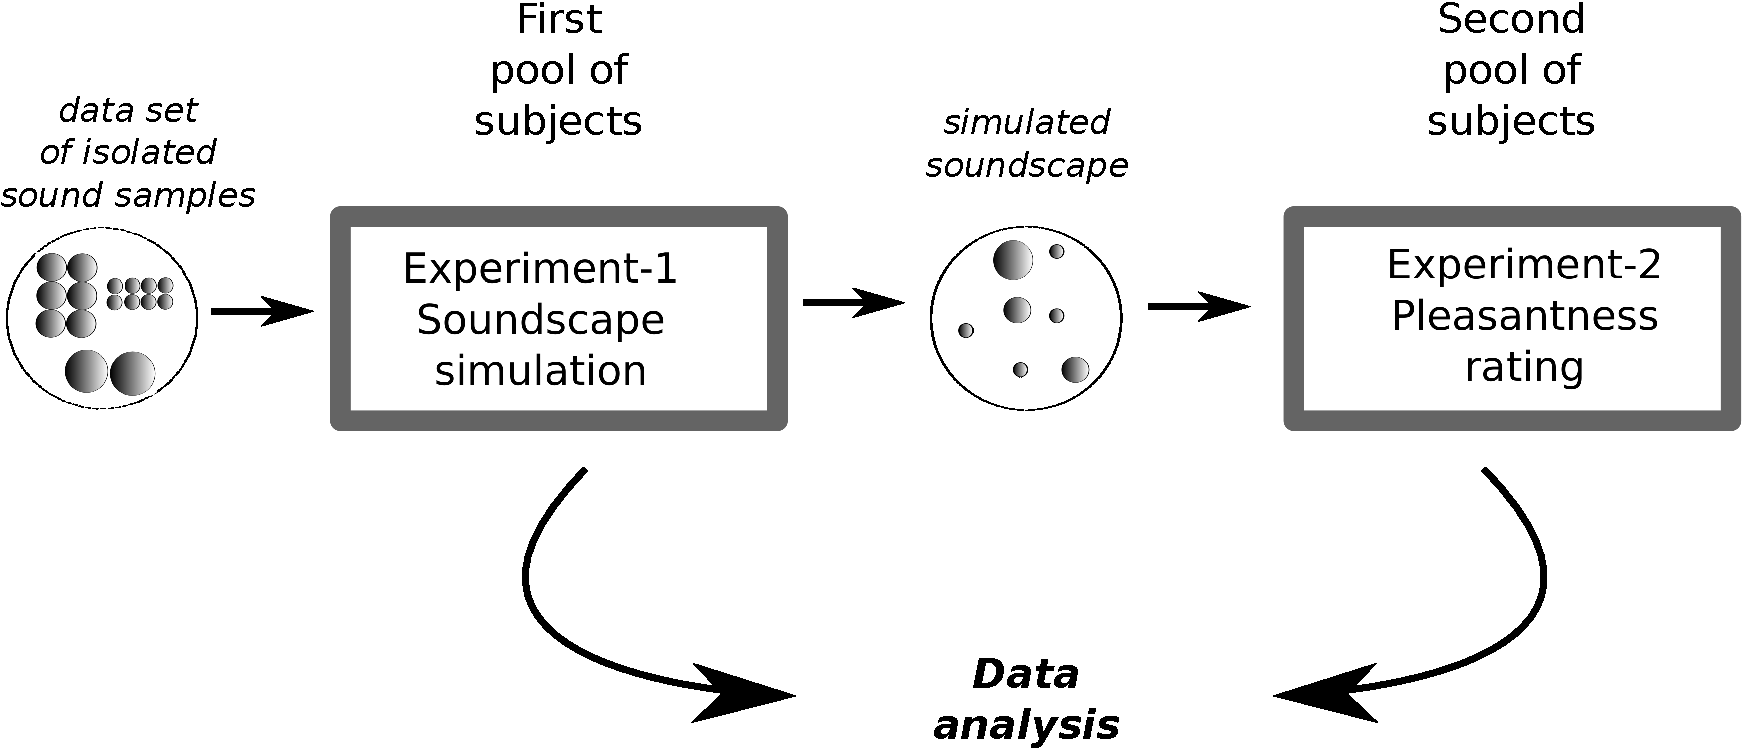
\includegraphics[width=.8\linewidth]{gfx/5-eps-converted-to}
        \caption{Planification expérimentales des éxperiences de simulation et d'évaluation de l'agrément}\label{fig:xp1_2}
\end{figure}

Cette expérience a fait l'objet d'une expérience pilote \citep{lafay2013atiam,lafay2014new}.

\subsection{Banque de données de sons isolés}

Dans cette section, nous présentons le processus de sélection et d'acquisition des sons isolés utilisés comme matériaux de base lors de la simulation des environnements sonores urbains. La banque de données est identique à celle utilisée dans le cadre de l'expérience pilote \citep{lafay2013atiam,lafay2014new}. Nous invitons le lecteur à se référer à la section~\ref{sec:db_ui} pour une description détaillée sur la manière dont les sons sont organisés dans la banque de données, ainsi que de l'interface permettant de les sélectionner. 

\subsection{Typologie des sources sonores présentes dans l'environnement urbain}

Dans le but de créer un corpus de sons isolés de référence pour la simulation, nous avons réalisé une typologie des sons environnementaux urbains. Dans un premier temps, les éléments présents dans cette typologie sont issus d’une étude bibliographique.

Nous recherchons les sources et ambiances sonores les plus souvent citées dans la littérature. Notre étude porte sur 16 articles ou thèses. Chacun d’eux traite de la manière dont nous discriminons les paysages sonores urbains. Plusieurs approches sont possibles, nous en avons relevés 3 :

\begin{itemize}
\item 9 articles abordent le problème par une approche perceptive, soit en identifiant ou répertoriant des catégories de sources sonores, soit en étudiant l'impact de classes de sons spécifiques sur la perception de l'environnement : \cite{maffiolo_caracterisation_1999,raimbault2002simulation,guastavino_etude_2003,defreville2004aactivity,raimbault2005urban,dubois2006cognitive,devergie_relations_2006,guastavino2006ideal,niessen2010categories}
\item 3 articles proposent une classification morpho-typologique, divisant l’environnement sonore urbain en ``\,zones sonores\,'' possédant une identité acoustique forte selon la configuration et la pratique du site : \cite{maffiolo_caracterisation_1999,beaumont2004pertinence,polack2008perceptive}
\item 2 articles répertorient et classifient les sources sonores d’un point de vu expert : \cite{leobon_analyse_1986,brown2011towards}
\end{itemize}

La nature des classes est établie par rapport aux catégories perceptives ou classes de sons les plus souvent citées dans ces papiers. A  partir des éléments relevés, nous établissons deux taxonomies : une pour les événements (\cf~Figure~\ref{fig:taxonomie}.a), et une pour les textures (\cf~Figure~\ref{fig:taxonomie}.b). Comme évoqué à la section~\ref{sec:db_ui}, la structure taxonomique de ces deux ensembles s'inspire grandement de l'axe verticale de l'organisation catégorielle comme proposée par E. Rosch (\Cf~section~\ref{XX}), \ie~plus le niveau d'abstraction de la classe est élevé, plus la description de la classe est précise et plus les source sonores appartenant à la classe sont semblables (\Cf~Figure~\ref{fig:orgDb}). Pour les événements, nous considérons 4 niveaux d'abstraction allant des classes les plus globalisantes (niveau d'abstraction 0) au classes les plus spécifiques (niveau d'abstraction 3). Pour les textures nous ne considérons que 3 niveau d'abstraction.

Nous notons que la typologie ainsi obtenue est très similaire à une autre typologie de sources sonores présentes en milieu urbain effectuée postérieurement \citep{Salamon14}. \\

\gl{Vérifier les articles que Salamon utilise pour établir sa typologie}

\begin{figure}[bth]
        \myfloatalign
        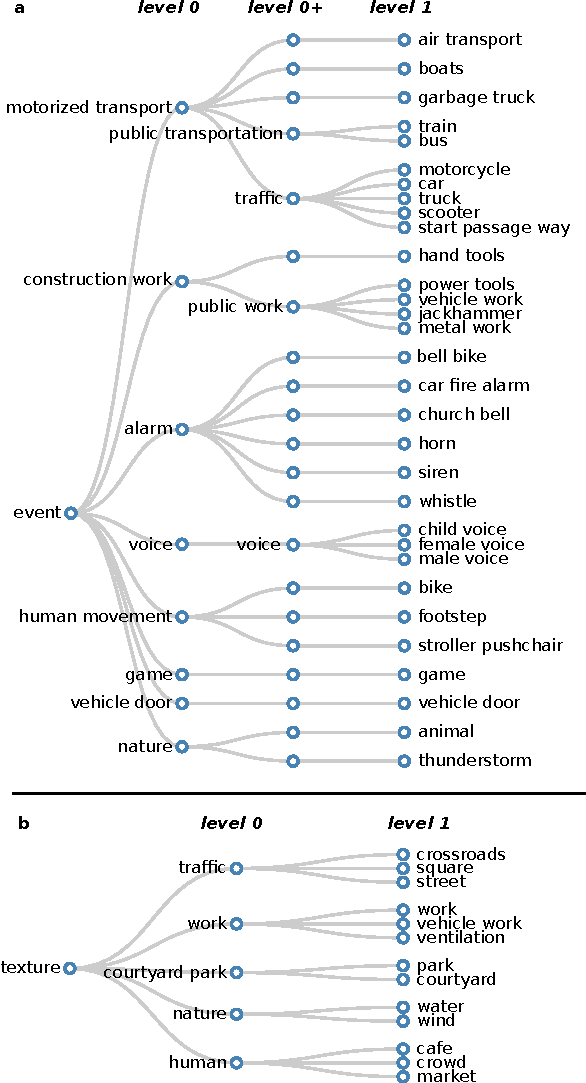
\includegraphics[width=.8\linewidth]{gfxHierarchy/taxonomy}
       \caption[Taxonomies des classes de sons utilisées pour la simulation des environnements sonores urbains]{Taxonomies des classes de sons utilisées pour la simulation des environnements sonores urbains pour (a) les événements sonores et (b) les textures sonores. Nous présentons ici uniquement les niveaux d'abstraction 0 et 1. Un niveau intermédiare, nommé $0+$ et utilisé pour l'analyse est également introduit.}\label{fig:taxonomie}
\end{figure}

\subsection{Acquisition des sons isolés}

Sur la base des typologies précédemment établies, nous avons collecté 483 sons, dont 381 des événements et 102 des textures.

Parmi les sons d'événements :

\begin{itemize}
\item 260 sont issus d’enregistrements
\item 89 sont issus de la banque de sons \emph{SoundIdeas}\footnote{Pour plus de détails sur \emph{SoundIdeas} voir :\url{ http://www.sound-ideas.com/}}
\item 32 sont issus de la banque de sons \emph{Universal SoundBank}\footnote{Pour plus de détails sur \emph{Universal SoundBank} voir : \url{http://www.universal-soundbank.com/}}
\end{itemize}

Parmi les textures:

\begin{itemize}
\item 72 sont issus d’enregistrements
\item 23 sont issus de la banque de sons \emph{SoundIdeas}
\item 7 sont issus de la banque de sons \emph{Universal SoundBank}
\end{itemize}

Tous les enregistrements ont été effectués à l’aide d'un micro canon \emph{AT8035}\footnote{\Cf~\url{http://eu.audio-technica.com/fr/products/product.asp?catID=1&subID=6&prodID=1845}} relié à un enregistreur \emph{ZOOM H4n}\footnote{\Cf~\url{http://www.zoom.co.jp/english/products/h4n/}}. L’utilisation du micro canon nous permet d’isoler les événements sonores du magma urbain. Inversement, pour les textures, il nous permet d’éviter les événements sonores proches du preneur de son, chose impossible avec un micro omnidirectionnel. Nous pouvons ainsi pointer des "zones sonores", en nous tenant à une certaine distance de ces dernières afin de capter uniquement le brouhaha émanant de la zone ciblée.

Tous les sons ont été normalisés au même niveau $RMS$ \footnote{Le niveau $RMS$, de l'anglais \emph{Root Mean Square} désigne la valeur efficace d'un signal. Formellement, le niveau $RMS$ $x_{RMS}$ d'un signal $x=(x_1,x_2,\ldots,x_n)$ s'obtient en calculant la moyenne quadratique de ce dernier $x_{RMS}=\sqrt{\dfrac{1}{n}\sum\limits_{i} x_i^2}$} de $-12$ $dB$ (FS) \footnote{$dB$ (FS) est le sigle anglais désignant une valeur en décibel relative à la pleine échelle (\emph{relative to Full Scale}), \ie~le rapport entre le niveau du signal et sa valeur maximale. Dans notre cas, ce niveau pleine échelle est de 1 Volt.}.

\subsection{Planification expérimentale}

\subsubsection{Épreuve de simulation}

\textbf{Procédure} \\

Les sujets doivent simuler deux environnements sonores urbains, chacun d'une durée de 1 minute.  Pour les deux simulations, les sujets doivent se conformer aux consignes suivantes.

\begin{itemize}
\item Première simulation : Simuler un paysage sonore \textbf{urbain plausible} qui selon vous est idéal (où vous aimeriez vivre).
\item Deuxième simulation : Simuler un paysage sonore \textbf{urbain plausible} qui selon vous est non-idéal (où vous n'aimeriez pas vivre).
\end{itemize}

Tous les sujets commencent par simuler l'environnement idéal. Les sujets ne prennent connaissance de la deuxième consigne qu'à la fin de la première simulation.

Les sujets son totalement libres dans le choix des sons, et des paramètres. Il doivent cependant se conformer à deux contraintes:

\begin{itemize}

\item Les sujets doivent mimer un auditeur statique.
 
\item Les environnements simulées doivent être plausibles, \ie~les sujets ne doivent pas simuler de situation physiquement irréalistes. L'exemple suivant d'une situation physiquement irréaliste est donné aux sujets: 

\begin{quote}
Un chien aboyant toutes les 10 millisecondes.
\end{quote}

\end{itemize}

Avant de commencer la première simulation, les sujets doivent réaliser un petit tutoriel de 20 minutes, afin de se familiariser avec le logiciel de simulation.

L'expérience est prévue pour durer 2h30. \\


\gl{description détaillée des étapes de simulation} \\


\textbf{Apparatus} \\

Tous les sujets passent l'expérience sur des machines identiques (\gl{description des machines}). L'audio est présenter en stéréophonie, par le biais de casques audio. Pendant le tutoriel,les sujets doivent ajuster le niveau sonore à un volume confortable. Ils ne peuvent le modifier par la suite.

Tous les sujets réalisent l'expérience simultanément. Ils sont répartis de manière égale dans trois pièces identiques, toutes possédant un environnement calme. Ils n'ont pas le droit de s'adresser la parole pendant l'expérience.

Trois expérimentateurs, un dans chaque pièce, sont présents durant la totalité de l'expérience, afin de contrôler le bon déroulement de cette dernière, et de répondre à d'éventuelles questions des sujets.  \\

\textbf{Participants} \\

44 étudiants (14 femmes) de L’École Centrale de Nantes ont participé à l'expérience. Ils ont tous un peu près le même âge (moyenne: 21.6, écart-type: 2). Tous les sujets ont vécu dans la même ville (Nantes), au minimum pendant les deux dernières années précédant l'expérience.

Dû a une incompréhension des consignes, ou à l'impossibilité de finir dans les temps, 4 sujets ne sont pas pris en compte pour l'analyse. 40 sujets ont réalisés l'expérience avec succès, nous fournissant ainsi 80 scènes sonores simulés, 40 idéals, et 40 non-idéals.

\subsubsection{Épreuve d'évaluation de l'agrément}

\textbf{Procédure} \\

Les sujets doivent évaluer l'agrément des 80 scènes sonores simulées. Dû à des contraintes de temps, les sujets n'évaluent que 30 secondes des scènes simulées (à l'origine d'une durée de 1 minute). Ces 30 secondes sont extraites à partir de la 15ème et jusqu'à la 45ème seconde des scènes simulées de 1 minute.

L'évaluation s'effectue sur une échelle sémantique bipolaire de 7 points allant de -3 (non-idéal/très désagréable) à +3 (idéal/très agréable). Avant de noter une scènes, les sujets doivent obligatoirement écouter les 20 premières secondes de cette dernière. Après la notation, ils sont libre de passer à la scènes suivante, avant la fin des 30 secondes.

Pour chaque sujet, les scènes sont présentées dans un ordre aléatoire. Les dix premières scènes permettent au sujet d'ajuster ses notes. Elles sont obligatoirement composées de 5 scènes idéales et 5 non-idéales. Ces dix premières scènes sont rejouées à la fin de l'expérience, et seules les notes données à la deuxième occurrence sont prises en compte. \\

\textbf{Apparatus} \\

Tous les sujets passent l'expérience sur des machines identiques (\gl{description des machines}). L'audio est présenté en stéréophonie, par le biais de casques audio semi-ouvert \emph{Beyer-Dynamic DT 990 Pro}. Toutes les scènes sonores ont été re-simulée sur la base des partitions (\gl{citer section décrivant le terme partition}) obtenues lors de l'expérience de simulation. Le niveau sonore de sortie est identique pour tous les sujets.

Tous les sujets réalisent l'expérience simultanément, dans un environnement calme. Ils n'ont pas le droit de s'adresser la parole pendant l'expérience.

Un expérimentateur est présent durant la totalité de l'expérience, afin de contrôler le bon déroulement de cette dernière, et de répondre à d'éventuelles questions des sujets.  \\

\textbf{Participants} \\

10 étudiants (2 femmes) de L’École Centrale de Nantes ont participé à l'expérience. Aucun d'entre eux n'a réalisé l'expérience de simulation. Tous les sujets ont un peu près le même âge (moyenne: 23.1, écart-type: 1.8). Tous les sujets ont vécu dans la même ville (Nantes), au minimum pendant les deux dernières années précédant l'expérience.

Tous les sujets ont réalisés l'expérience avec succès.

\subsection{Données et méthodes d'analyses}

\subsubsection{Nature des données analysées}

Chaque scène est décrite par un groupe de descripteurs. C'est sur la base de ces descripteurs que nous pratiquons l'analyse. Un résumé des descripteurs, ainsi que des acronymes les désignant est présenté dans le Tableau~\ref{XX}.

Les descripteurs sont calculés sur chaque scène sonore. Nous considérons trois types de descripteurs:

\begin{itemize}
\item \emph{Perceptif}: Il s'agit de l'agrément perçu des scènes simulées, évalué sur une échelle sémantique 7 points. Nous notons $A$ l'agrément moyen d'une scène, obtenu en moyennant les notes de tous les sujets. Considérant le faible nombre de sujets, nous faisons le choix dans cette étude de ne pas normaliser les notes d'agrément.
\item \emph{Sémantique}: Il s'agit d'un vecteur booléen noté $S=(x_1,x_2,\ldots,x_n)$ indiquant les classes de sons présentes dans la scènes. Chaque point $x$ de ce vecteur correspond à une classe de son particulière: $x=1$ si la classe est présente dans la scènes, et $x=0$ autrement. La dimension $n$ des vecteurs dépend ainsi du niveau d'abstraction considéré, \eg~pour le niveau d'abstraction 1, qui comprend $44$ classes de sons, cette dimension sera de $n=44$.
\item \emph{Structurel}: Les descripteurs structurels sont calculés à partir des partitions et des signaux des scènes simulées. Trois descripteurs structurels sont envisagés:
\begin{itemize}
\item \emph{Diversité} ($DIV$) : Il s'agit d'un scalaire représentant la diversité des classes sonores utilisées pour simuler une scènes. Nous calculons $DIV$ en comptant le nombre de classes de sons distinctes utilisées pour une simulation. Ce nombre dépend du niveau d'abstraction considéré. Considérons les 2 sous classes du niveau d'abstraction 2 \emph{passage de voiture} et \emph{démarrage de voiture}, toutes deux appartenant à la classe \emph{voiture} du niveau d'abstraction 1, nous comptons 2 classes pour la diversité des niveaux d'abstraction 2 et 1, et seulement 1 pour les niveaux d'abstraction 0 et 1.
\item \emph{Densité} ($D$) : Il s'agit d'un scalaire représentant le nombre de source sonore présentes en moyenne. Pour obtenir $D$, nous calculons le logarithme du nombre d'éléments sonores par fenêtre de 125 millisecondes (sans recouvrement) et moyennons au cours du temps. Le calcul de $D$ peut inclure toutes les sources sonores de la scènes, ou seulement une partie. Dans ce cas, les fenêtres ne contenant pas de sources sonores ne sont pas prises en compte. Nous notons $DE$ et $DT$ les densités calculées en considérant séparément les source d'événements et de textures sonores respectivement.
\item \emph{Niveau Sonore} ($L$) : Pour représenter le niveau sonore, nous nous inspirons du la mesure $L_{Aeq}$. Dans notre cas, il s'agit d'un scalaire, calculé sur le signal en volt et non en pression, et donné en décibel en prenant un référentiel de 1 Volt. Le niveau est obtenu en calculant toutes les secondes la moyenne quadratique du signal, et en moyennant sur la durée de la scène. Un filtrage de type A est opéré avant le calcul des moyennes quadratiques. D'autre descripteurs inspirés eux aussi de descripteurs acoustiques classiques ($L_{Amin}$, $L_{Amax}$, $L_{A10-90}$), et utilisant un opérateur autre que la moyenne (minimum, maximum, les 10-90ème quantiles) pour intégrer les fenêtres de 1 seconde  ont été testés. Mais ces derniers présentant tous une corrélation élevé avec $L$ ($r_{pearson}\geq0.76$, $p<0.01$), nous conservons uniquement ce dernier comme descripteur objectif du niveau sonore.
\end{itemize}
\end{itemize}

\gl{tableau résumé des descripteurs}

\subsubsection{Méthodologie et Outils statistiques}


L'objectif de l'étude est d'évaluer l'impact spécifique des différentes sources sonore sur l'agrément perçue via l'utilisation de scènes simulées. Afin de répondre à cette question, nous divisons l'étude en 6 sous-objectifs:

\begin{itemize}
\item \emph{Étude qualitative} : Afin de vérifier la validité écologique de 1) la banque de données et 2) l'interface de sélection, nous réalisons une étude qualitative des commentaires libres des sujets effectués après l'épreuve de simulation.
\item \emph{Étude comparative entre les descripteurs structurels} : Il s'agit ici d'évaluer si la distinction affective imposée entre les i- et ni-scènes a impacté de manière significative la nature des scènes, \ie~si il existe des différences significatives entre les descripteurs structurels et/ou l'agrément perçu. La significativité est évaluée à partir d'un test de Student à échantillons apparié (\Cf~Annexe~\ref{app:statuni}).
\item \emph{Influence des descripteurs structurels sur l'agrément perçu}: Nous adoptons ici une méthodologie couramment utilisée dans l'approche dimensionnelle. Pour évaluer l'impact potentiel des descripteurs structurels sur l'agrément perçu, nous étudions l'existence de corrélation linéaire entre entre ces deux types de descripteur. Pour mesurer la corrélation, nous utilisons le coefficient de Pearson (\Cf~Annexe~\ref{app:statuni}).
\item \emph{Étude comparative entre les descripteurs sémantiques}: Il s'agit ici d'apprécier si la distinction affective imposée a eu un impact sur la composition des scènes en terme de sources sonores. Plus précisément, il s'agit d'observer si il existe des classes de sons qui ont été particulièrement utilisées pour simuler un type d'environnement. Nous utilisons le V-test afin de tester si la présence d'une classe de son est caractéristique d'un environnement (i ou ni) en particulier. Ces classes caractéristiques sont nommées les marqueurs sonores
\item \emph{Étude des espaces de représentations induits par les descripteurs sémantiques}: Dans cette analyse, nous étudions si une représentation basée uniquement sur la présence ou l'absence des classes de sons permets de séparer les deux types d'environnements. Pour ce faire nous considérons l'espace induit par les descripteurs sémantiques $S$. $S$ étant un vecteur booléen, nous calculons les distances entre les scènes à partir de la distance de \emph{hamming}. Considérant les deux vecteurs $S_1=(x_{1,1},x_{1,2},\ldots,x_{1,n})$ et $S_2=(x_{2,1},x_{2,2},\ldots,x_{2,n})$ de dimension $n$, avec $x={0,1}$, la distance de \emph{Hamming} $d_{ham}$ mesure le pourcentage de coordonnés qui diffèrent entre les deux vecteurs. 


\begin{equation*}
d_{ham}(S_1,S_2)=\dfrac{1}{n}\sum_{i=1}^{n} (x_{1,i} \bigoplus x_{2,i})
\end{equation*}

où $\bigoplus$ désigne l'opérateur du \emph{ou-exclusif}. Plus la composition des deux scènes est similaire, et plus ces deux scènes seront proches. L'utilisation de la distance de \emph{Hamming} permet de prendre en compte de manière égale les classes présentes et absentes. Pour mesure la capacité intrinsèque de l'espace à séparer les i- et ni-scènes nous utilisons une métrique de \emph{clustering} nommé précision au rang $k$ ($p@k$). Pour calculer la $p@k$, on regarde d'abord pour chaque item, le taux d'items partageant le même label parmi ses $k$ plus proche(s) voisin(s). La $p@k$ est alors la moyenne des taux pour tous les items.

\item \emph{Influence spécifique marqueurs sonore sur l'agrément perçu}: Une fois les marqueurs sonores identifiés, nous évaluons une nouvelle fois l'impact potentiel des descripteurs structurels sur l'agrément perçu, mais en ne tenant compte cette fois que des marqueurs sonores pour calculer ces descripteurs.
\end{itemize}

Tous les test de significativité sont effectués avec un seuil critique $\alpha=0.05$. Dans le cas ou la valeur $p\geq0.05$, nous indiquons sa valeur. Dans le cas ou $0.01\leq p<0.05$ nous indiquons seulement $p<0.05$. Dans le dernier cas nous indiquons $p<0.01$.

\subsection{Validité écologique de l'expérience}

\subsubsection{Diversité de la banque de sons}

Nous cherchons dans un premier temps à vérifier que les classes de sons proposées dans la banque de données soient assez diversifiée pour pouvoir simuler un environnent sonore. En analysant les commentaires des sujets portant sur la banque données, nous remarquons que 63\% des sujets ont indiqué avoir été au moins une fois dans l'incapacité de trouver un son, avec un maximum de 4 sons par sujet. Parmi tous les sons manquant relevés, nous avons identifié 26 classes de sons. Parmi ces 26 classes de sons manquantes:

\begin{itemize}
\item  16 sont bien présentes dans la banque de données, l'incapacité des sujets à les trouver n'étant donc pas imputable à la diversité de la base.
\item 1 fait référence a des sons de musique, que nous avons choisis délibérément d'occulter.
\item 9 sont effectivement absentes.  
\end{itemize}

Parmi les 9 classes de sons identifiées comme manquantes, nous observons que ces classes sont très spécifiques (\eg~\emph{voiture de sport} ou \emph{voix d'adolescent}), et peuvent ainsi être remplacé par des classes similaires (\eg~\emph{voiture} ou \emph{voix d'enfant} ou \emph{voix d'adulte}). Nous pensons que ces résultats montrent que la diversité proposée par la banque de sons est suffisante dans le cadre de notre étude.

\subsubsection{Facilité d'utilisation de l'interface de sélection}

En considérant les retours sur l'interface de sélection, nous observons que $32.5\%$ des sujets ont spontanément indiqué que l'interface était un moyen ``\,simple et efficace\,'' de sélectionner des sons sans l'aide de texte. $57.5\%$ des sujets n'ont pas fait mention de difficulté particulière. Seulement $10\%$ des sujets ont signalé avoir rencontré des difficultés avec l'interface, mais sans que ces dernières aient sensiblement affecté la simulation.

Ces résultats tendent à montrer que l'interface de sélection sans texte n'a pas perturbé les sujets outre mesure. Des conclusions similaires ont été obtenues lors de l'expérience pilote \citep{lafay2013atiam,lafay2014new}. \\

\gl{vérifier une dernière fois}

\subsection{Vérification de l'agrément des scènes simulées}

Nous analysons ici l'agrément perçu des $80$ scènes sonores simulées. 

La Figure~\ref{fig:xp2_Aa} affiche agrément moyen $A$ pour les i- et ni-scènes. Afin de garantir la cohérence de nos données, nous voulons dans un premier temps nous assurer qu'aucune ni-scène n'ait un $A$ supérieur à celui d'une i-scène. Nous observons la Figure~\ref{fig:xp2_Aa} que quatre scènes ont une notation qui ne respecte pas cette contrainte. Ces scènes, ainsi que le correspondante i ou ni, sont supprimées de l'analyse, nous laissant ainsi avec 36 i-scènes et 36 ni-scènes.

Dans un second temps nous testons si les sujets ont bien perçu une différence d'agrément entre les i- et ni-scènes. Pour ce faire, nous observons l'agrément moyen de chaque sujet calculé séparément pour chaque type d'environnement (\Cf~Figure~\ref{fig:xp2_Ab}). Il est clair que les i-scènes ont bien été perçues comme significativement plus agréables ($p<0.01$) que les ni-scènes.

\begin{figure}[bth]
        \myfloatalign
        \subfloat[]
        {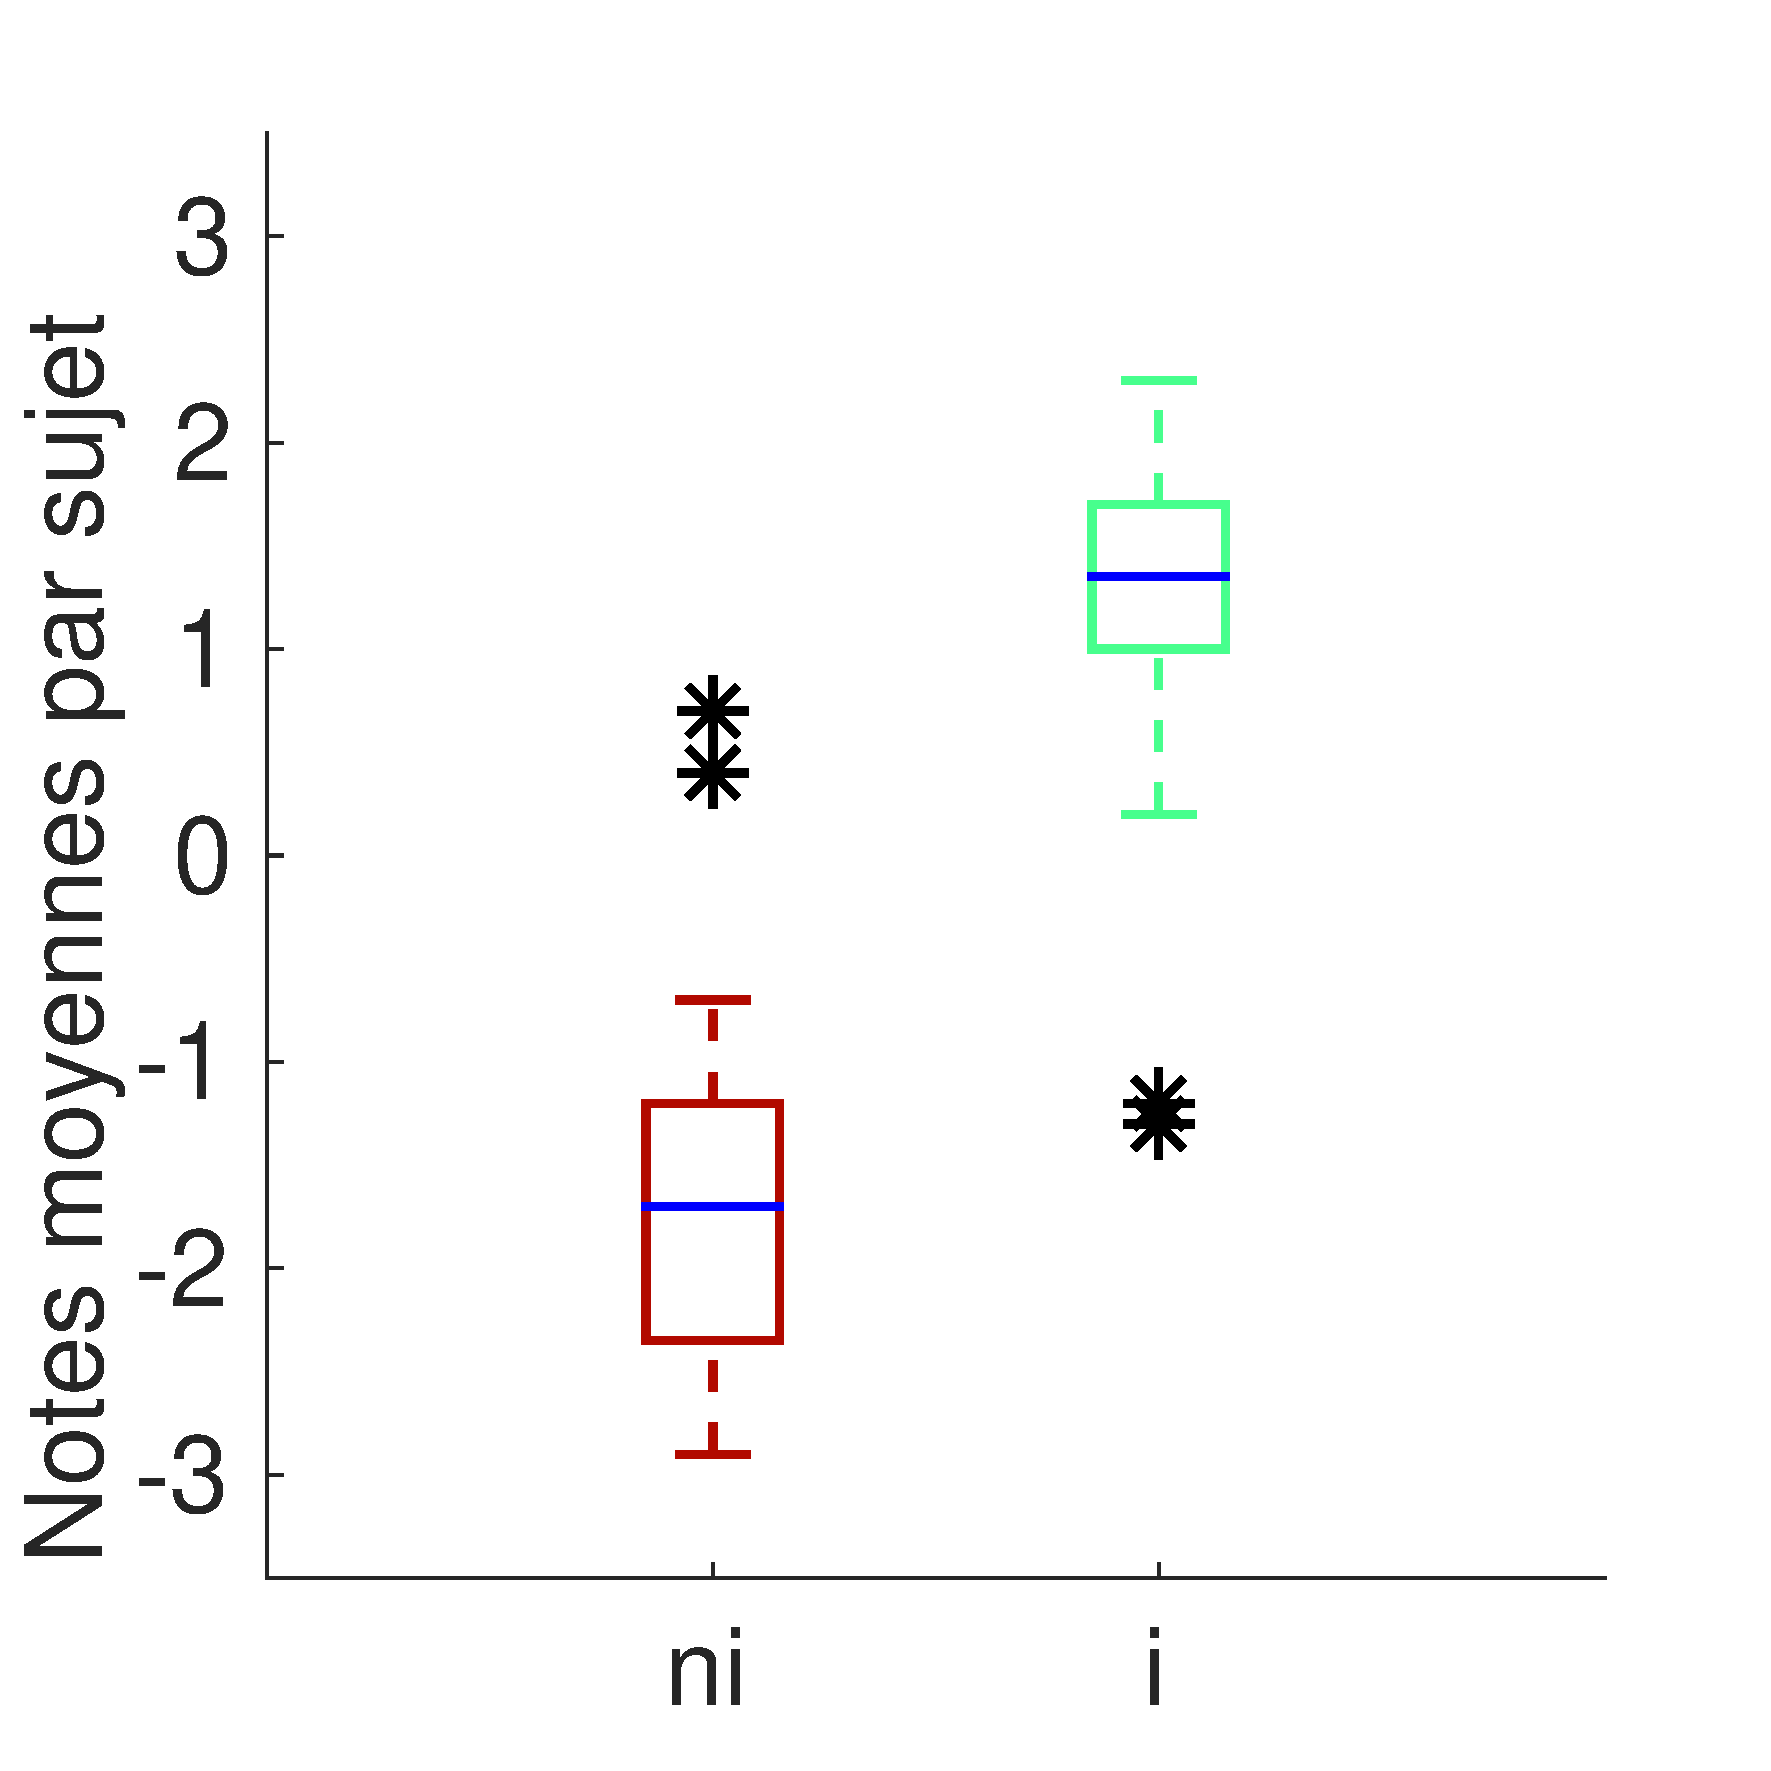
\includegraphics[width=.5\linewidth]{gfxXpUrbanSoundscape/xp2_1}\label{fig:xp2_Aa}}
        \subfloat[]
        {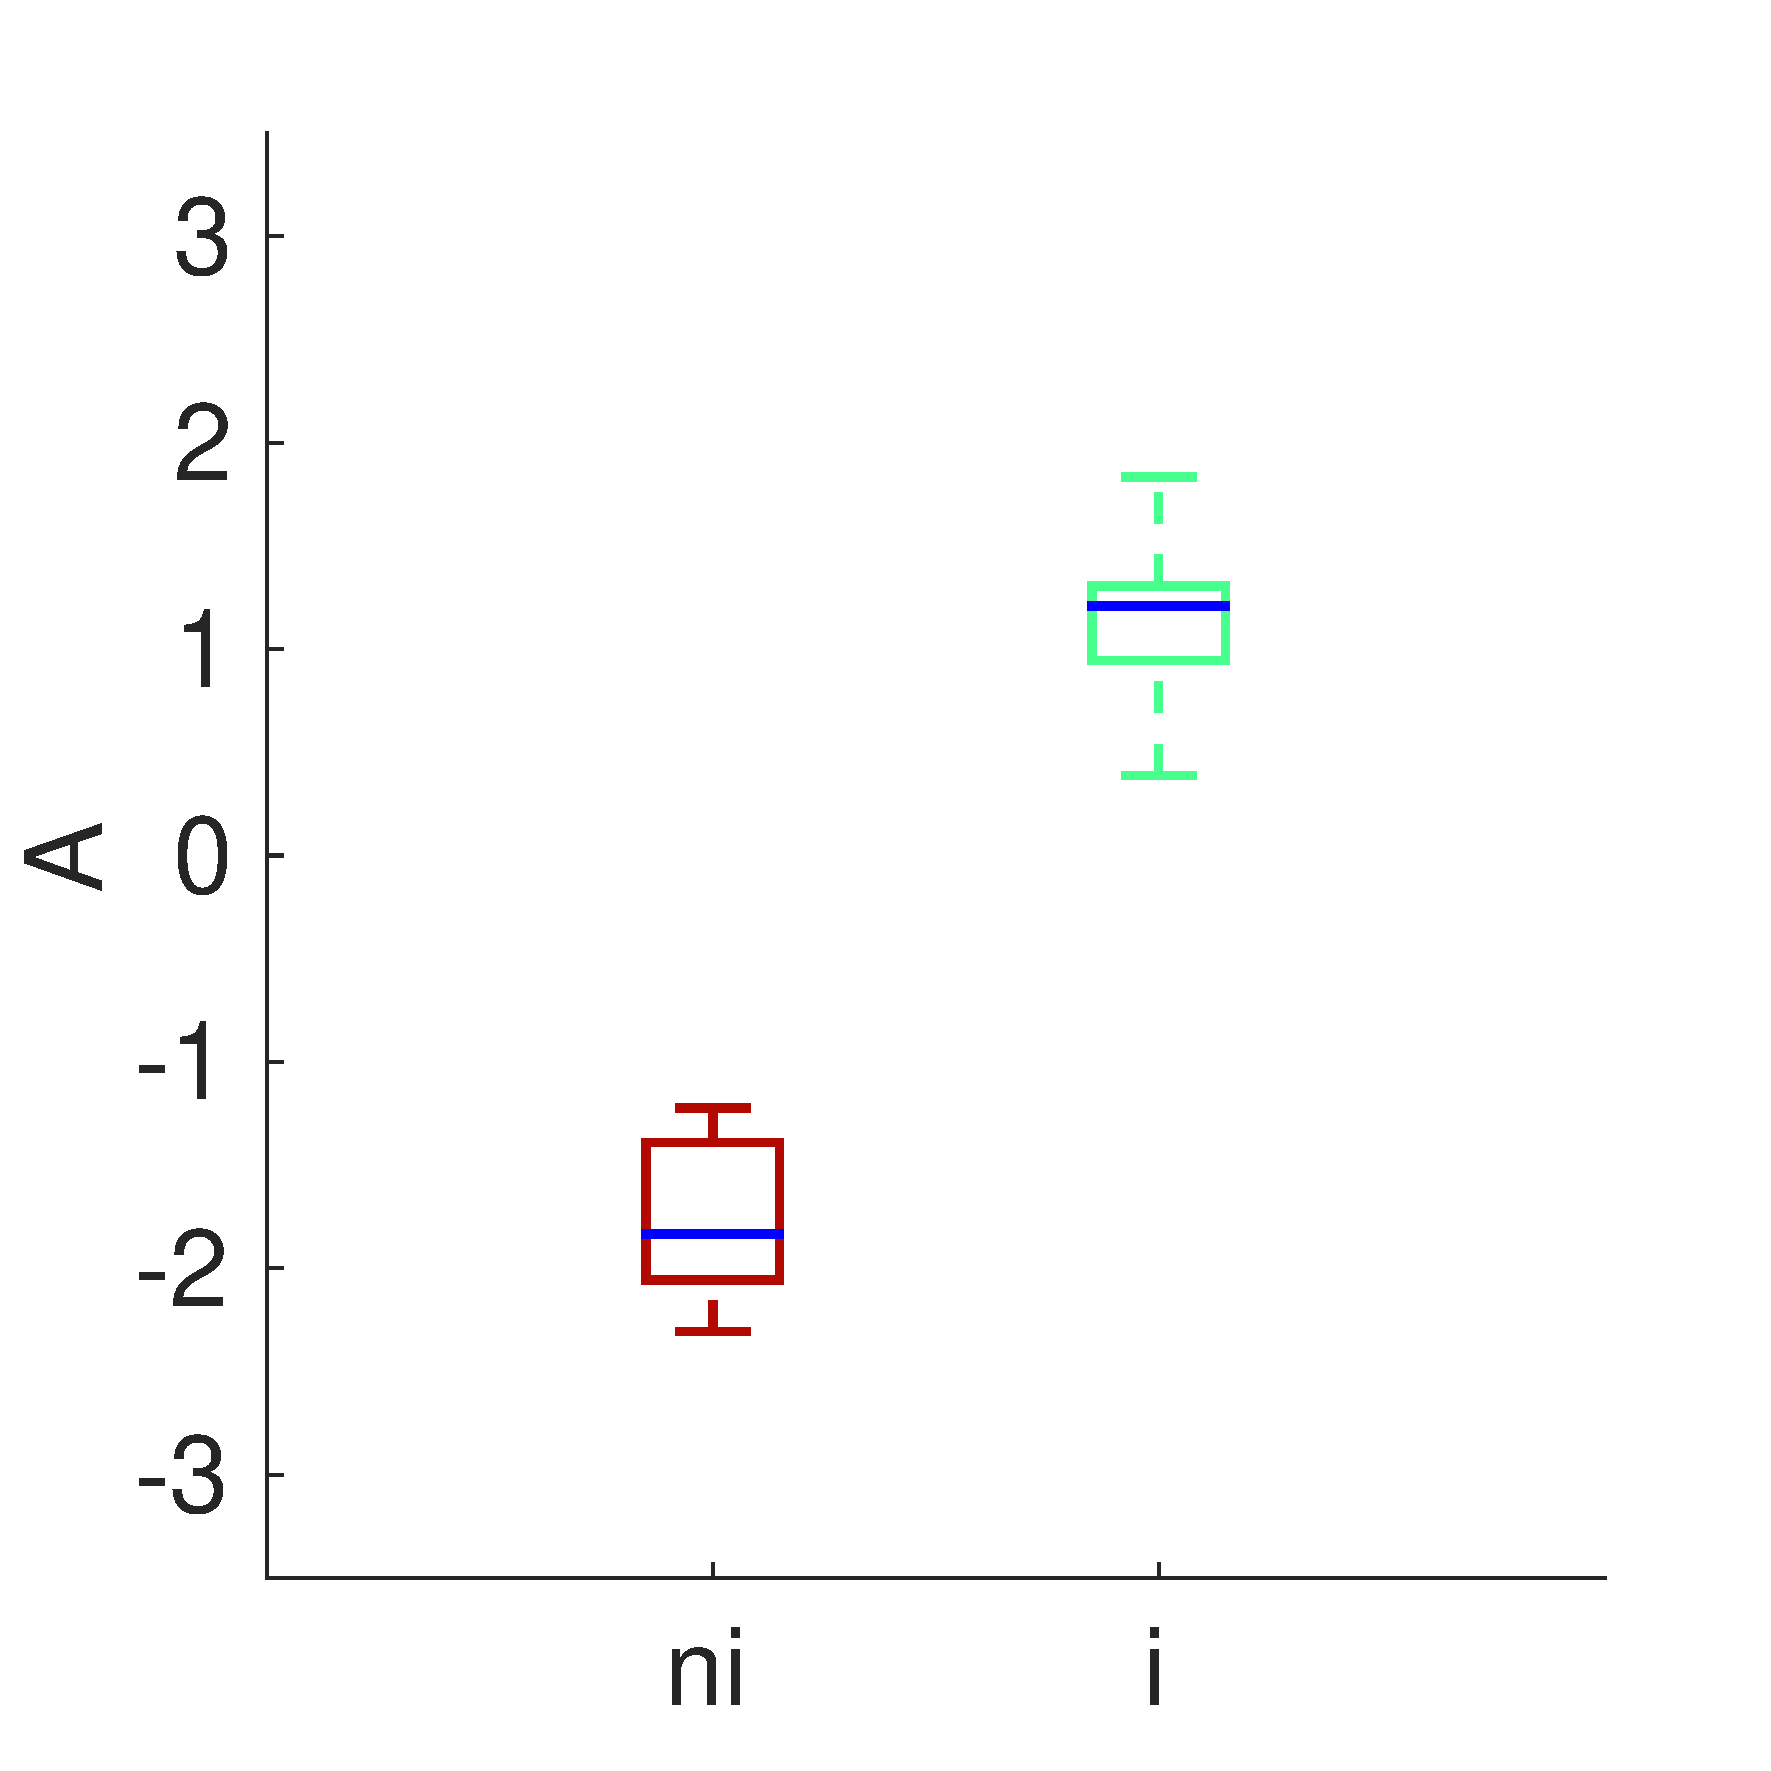
\includegraphics[width=.5\linewidth]{gfxXpUrbanSoundscape/xp2_2}\label{fig:xp2_Ab}}
       \caption[TODO]{TODO}\label{fig:xp2_A}
\end{figure}
 
\subsection{Étude comparative entre les descripteurs structurels}

\begin{figure}[bth]
        \myfloatalign
        \subfloat[]
        {\includegraphics[width=.33\linewidth]{gfxXpUrbanSoundscape/xp_soundlevel_1}\label{fig:soundlevela}}
        \subfloat[]
        {\includegraphics[width=.33\linewidth]{gfxXpUrbanSoundscape/xp_soundlevel_3}\label{fig:soundlevelb}}
        \subfloat[]
        {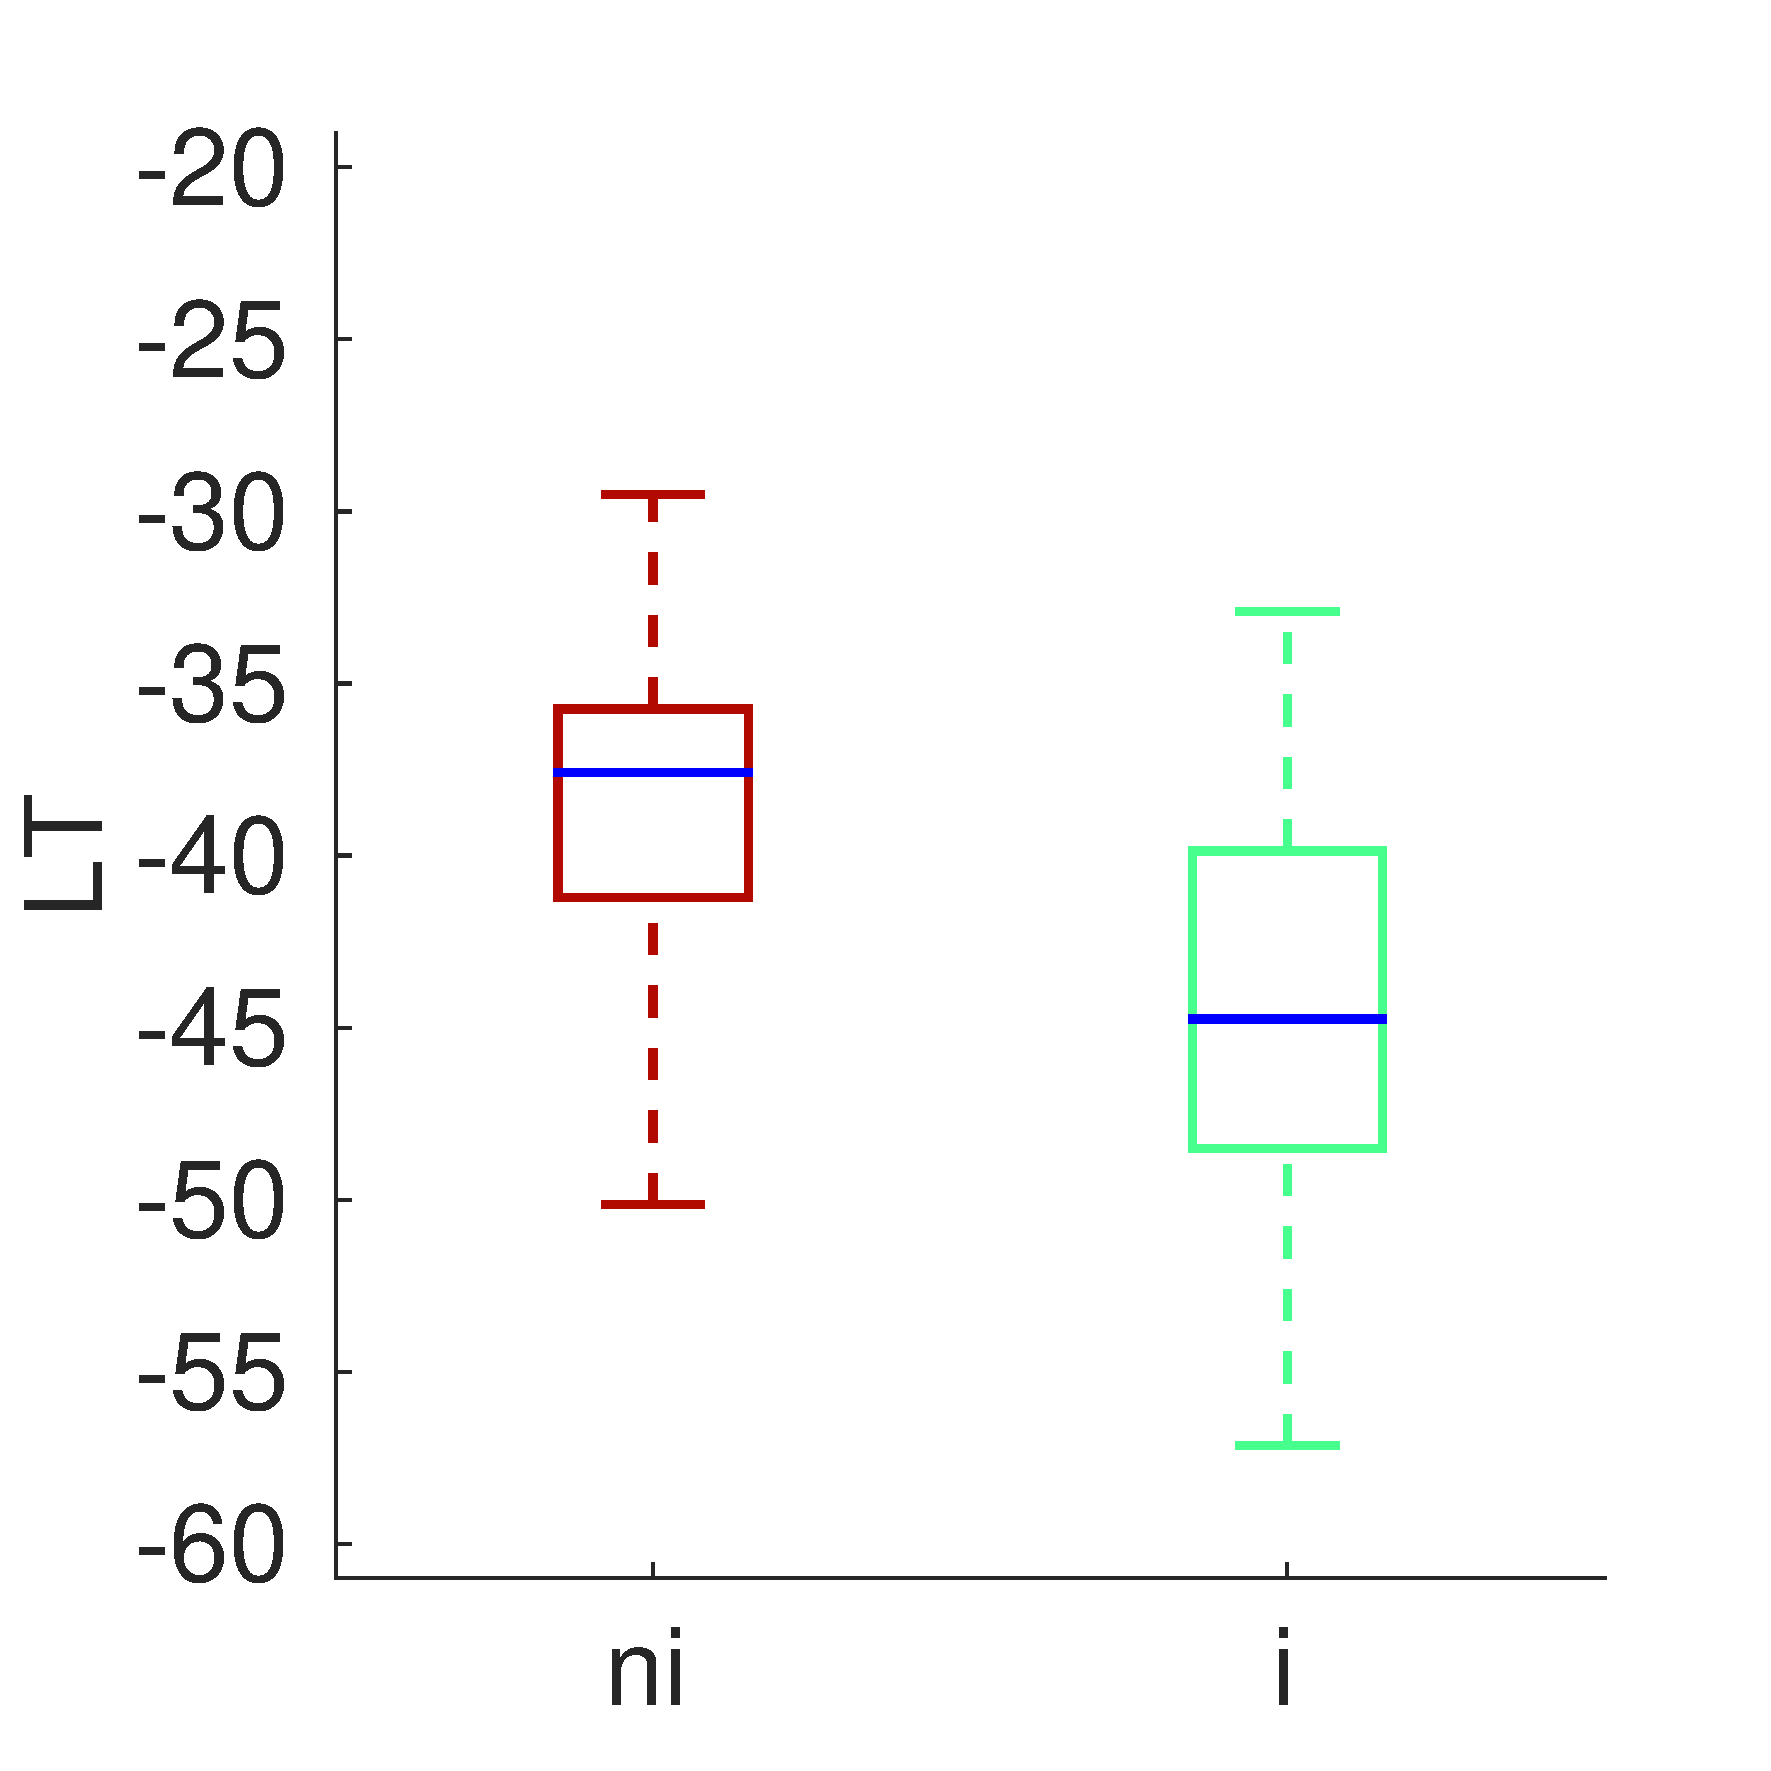
\includegraphics[width=.33\linewidth]{gfxXpUrbanSoundscape/xp_soundlevel_5}\label{fig:soundlevelc}}\par
        \subfloat[]
        {\includegraphics[width=.33\linewidth]{gfxXpUrbanSoundscape/xp_soundlevel_2}\label{fig:soundleveld}}
        \subfloat[]
        {\includegraphics[width=.33\linewidth]{gfxXpUrbanSoundscape/xp_soundlevel_4}\label{fig:soundlevele}}
        \subfloat[]
        {\includegraphics[width=.33\linewidth]{gfxXpUrbanSoundscape/xp_soundlevel_6}\label{fig:soundlevelf}}
       \caption[TODO]{TODO}\label{fig:soundlevel}
\end{figure}

\begin{figure}[bth]
        \myfloatalign
        \subfloat[]
        {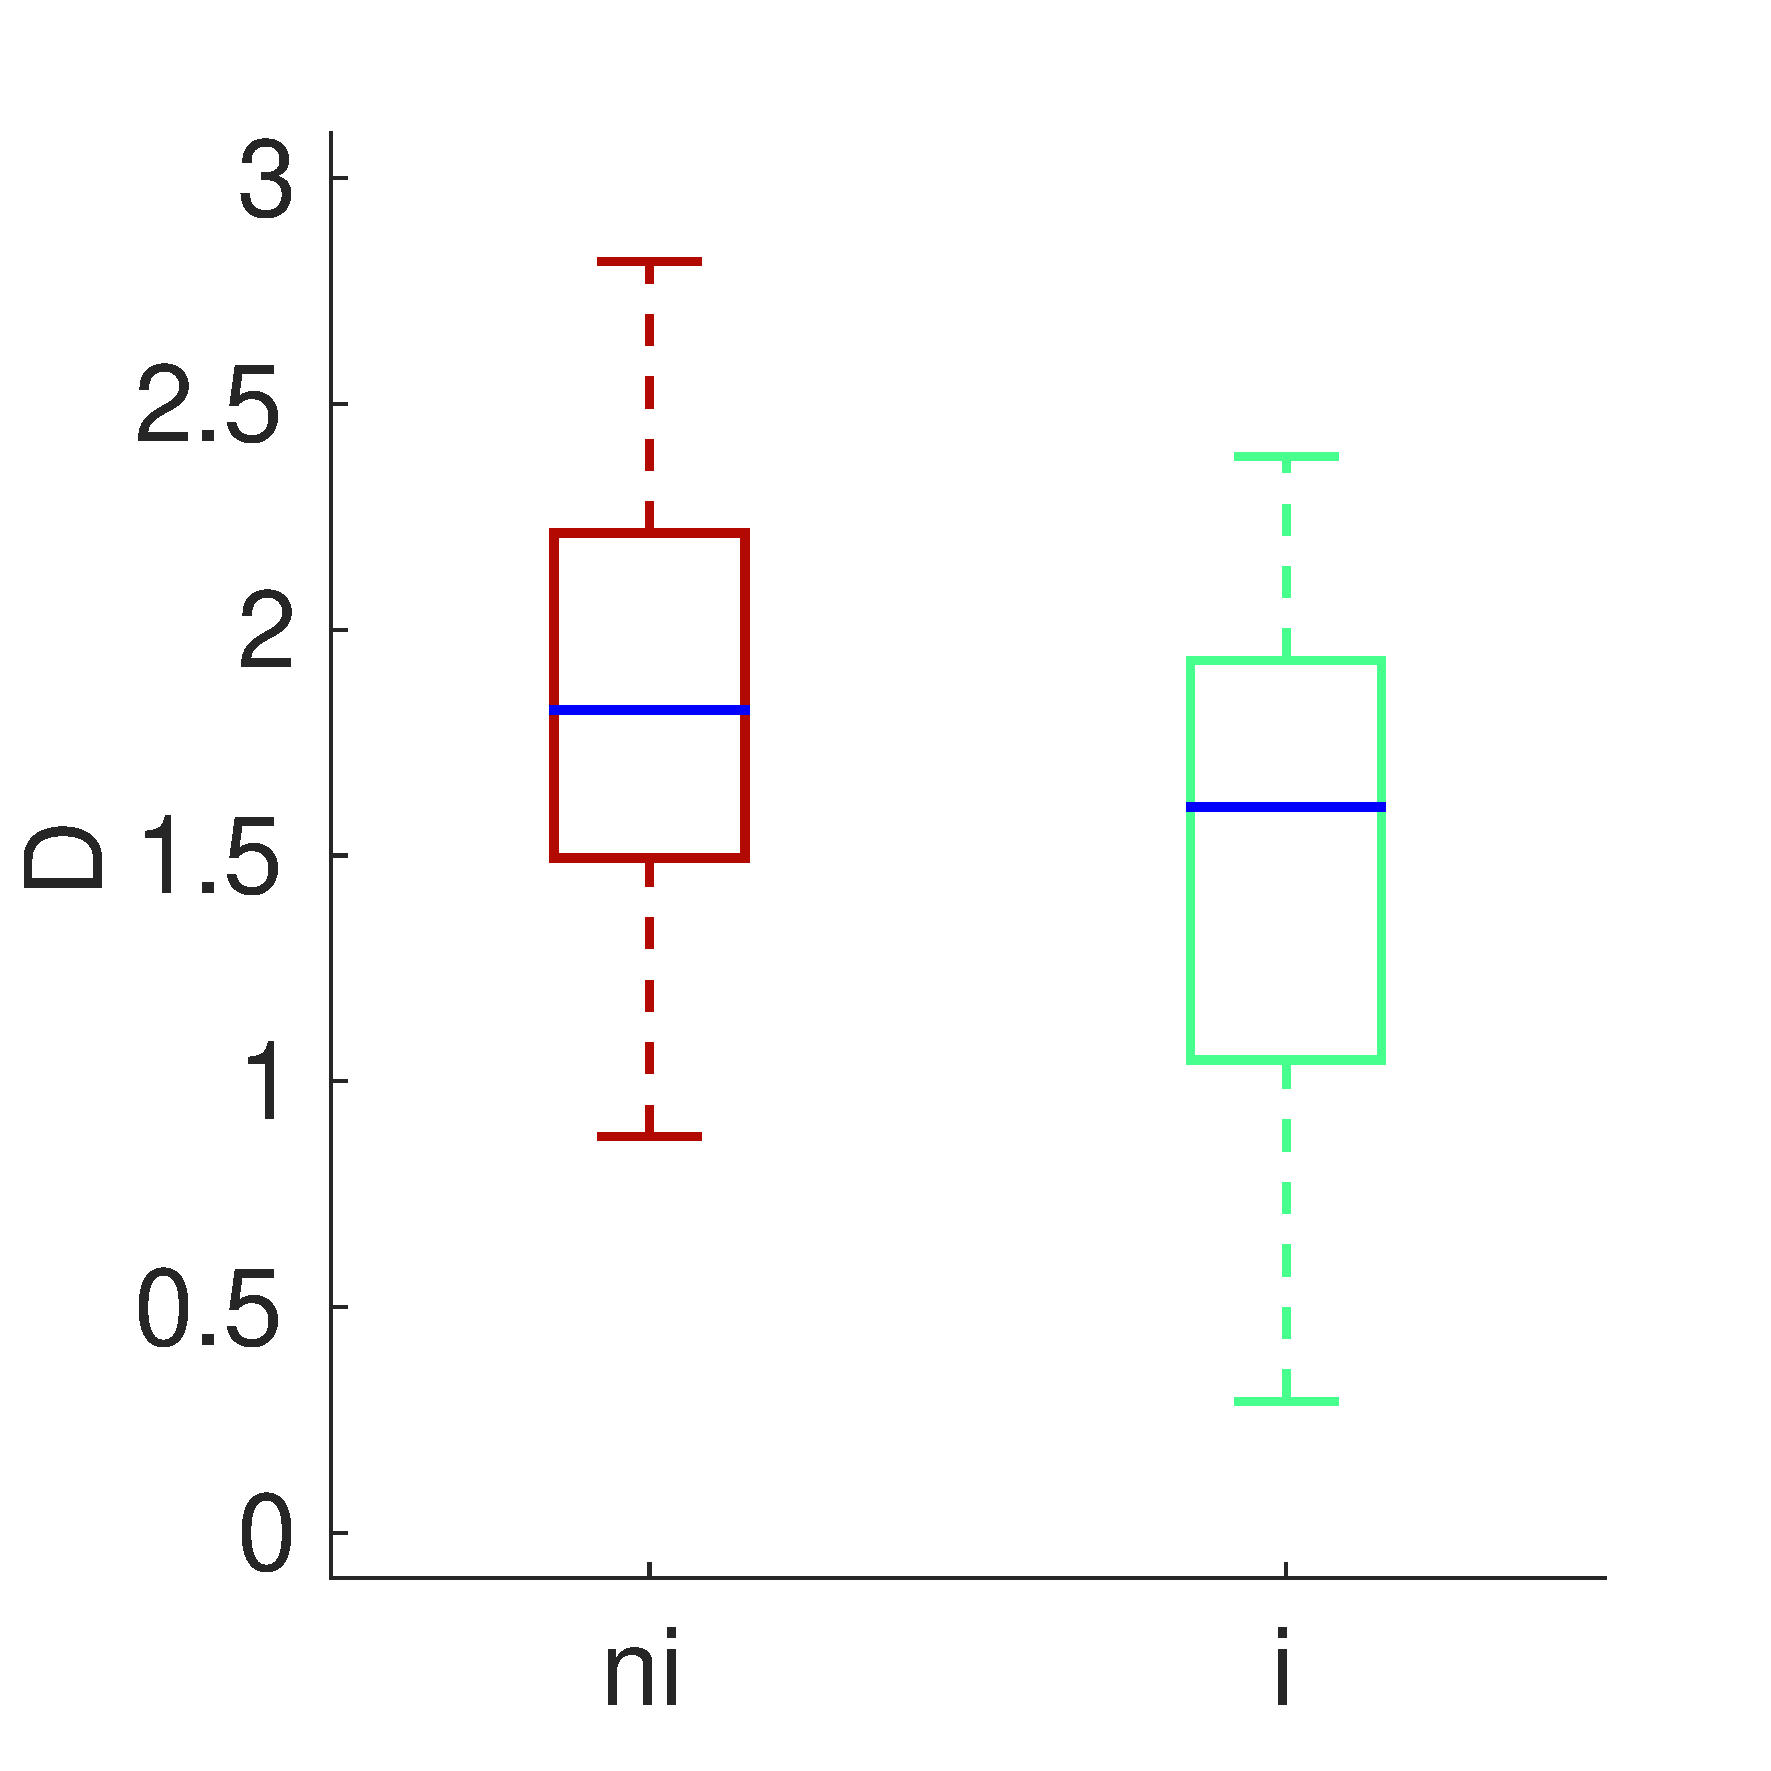
\includegraphics[width=.33\linewidth]{gfxXpUrbanSoundscape/xp_density_1}\label{fig:densitya}}
        \subfloat[]
        {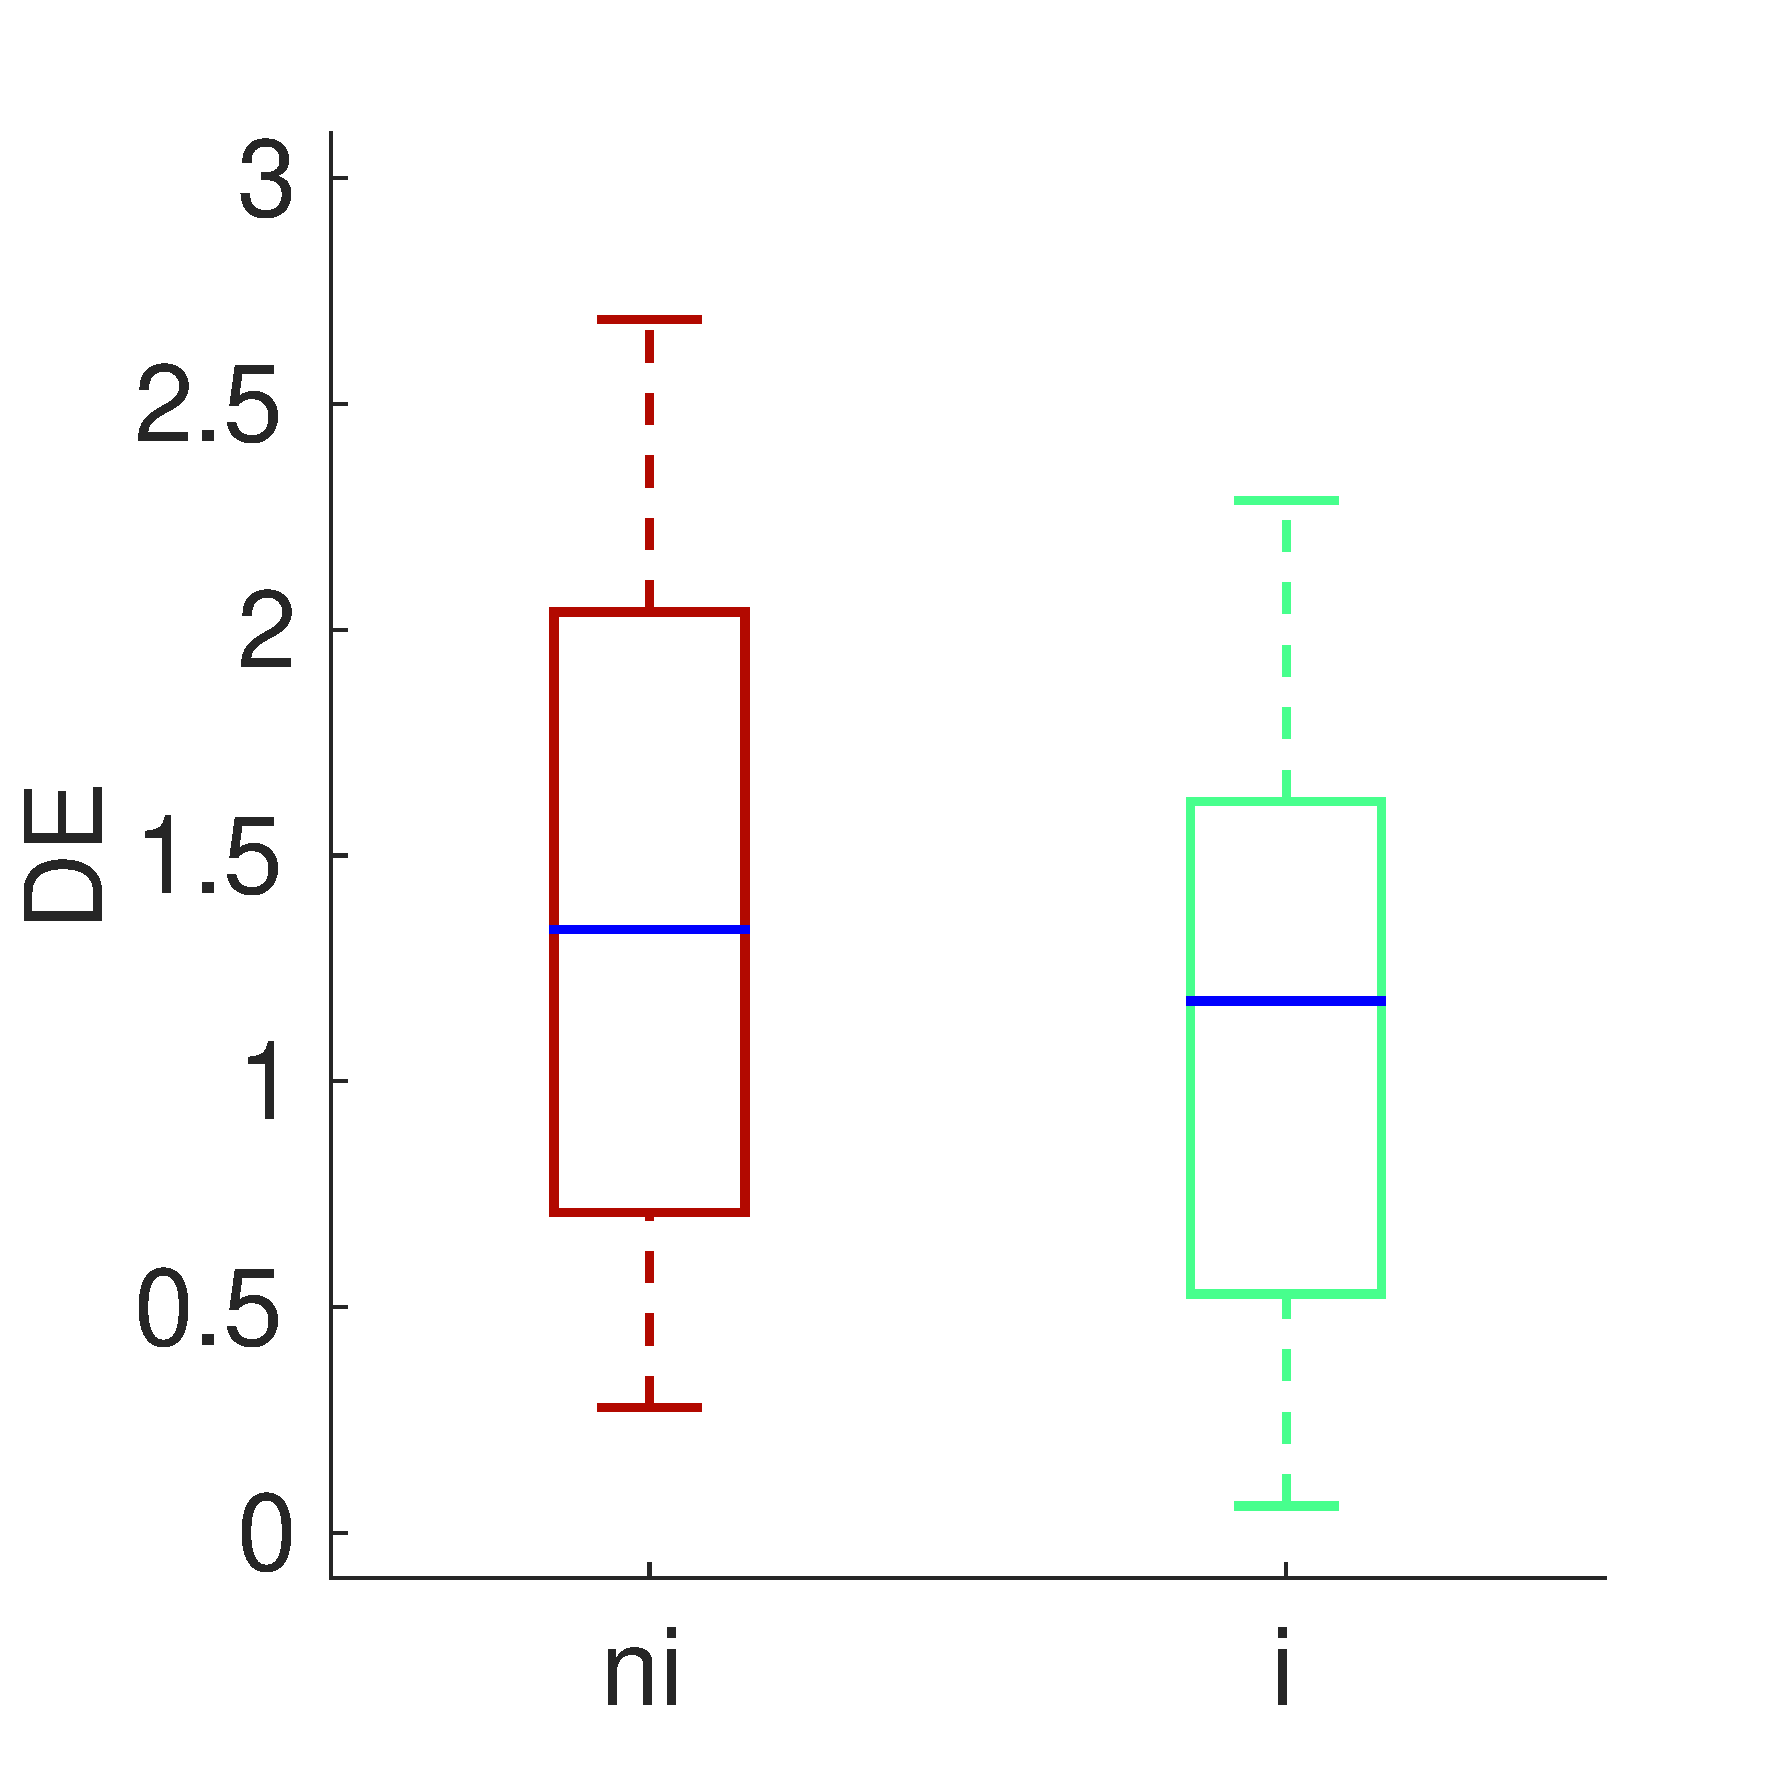
\includegraphics[width=.33\linewidth]{gfxXpUrbanSoundscape/xp_density_3}\label{fig:densityb}}\par
        \subfloat[]
        {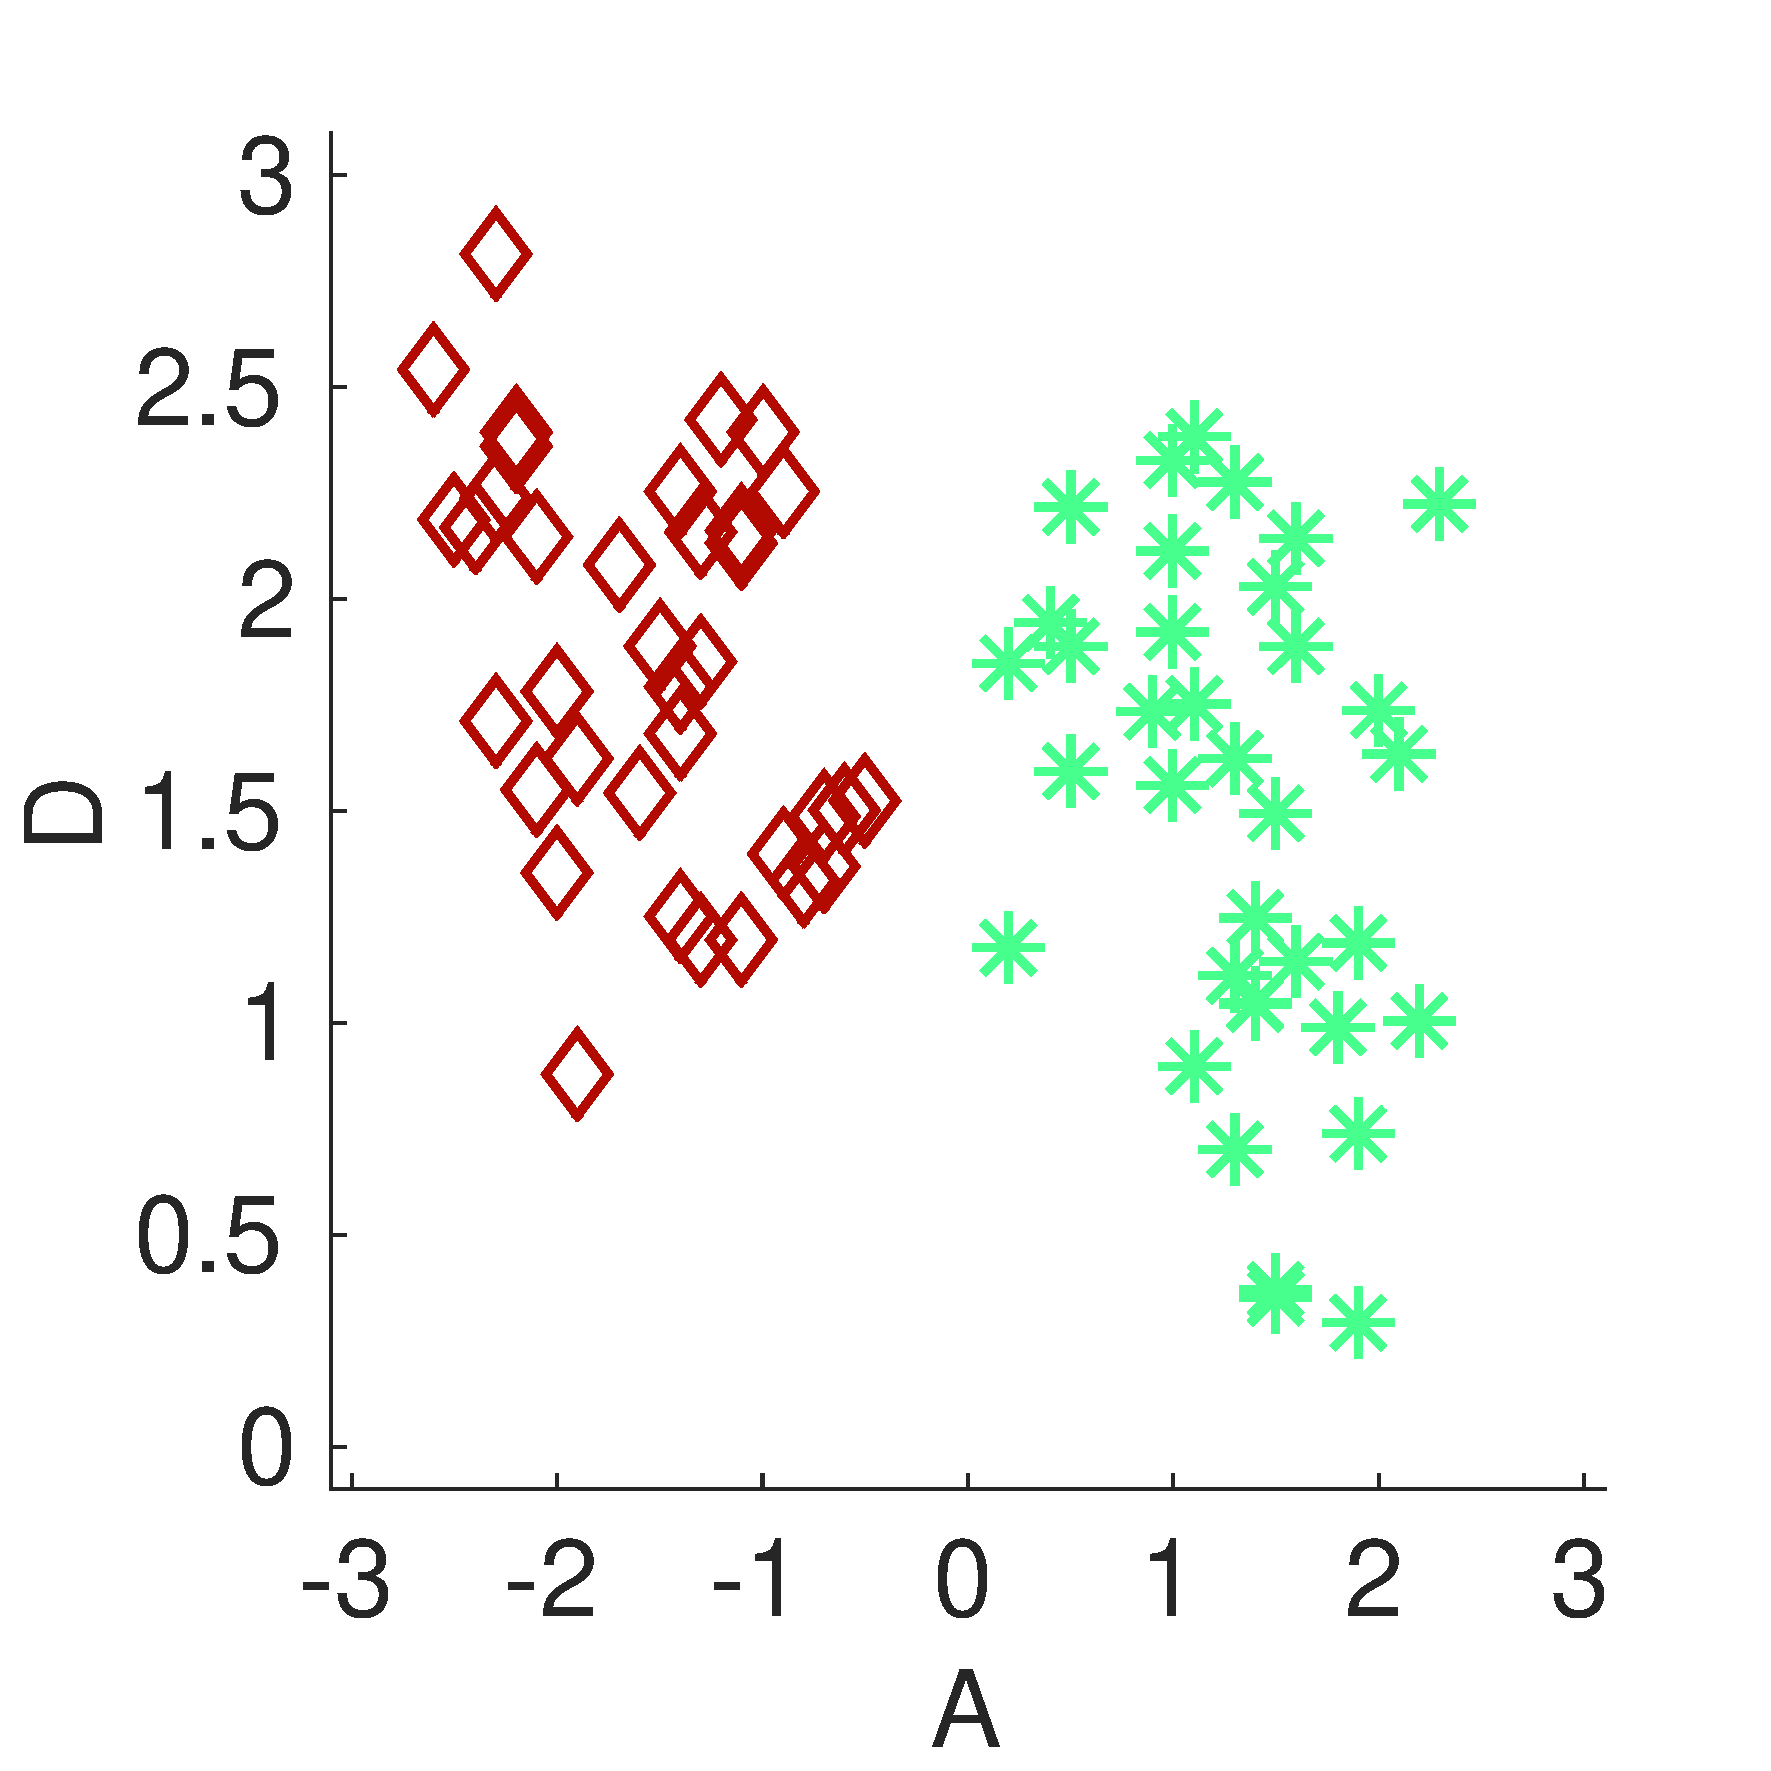
\includegraphics[width=.33\linewidth]{gfxXpUrbanSoundscape/xp_density_2}\label{fig:densityc}}
        \subfloat[]
        {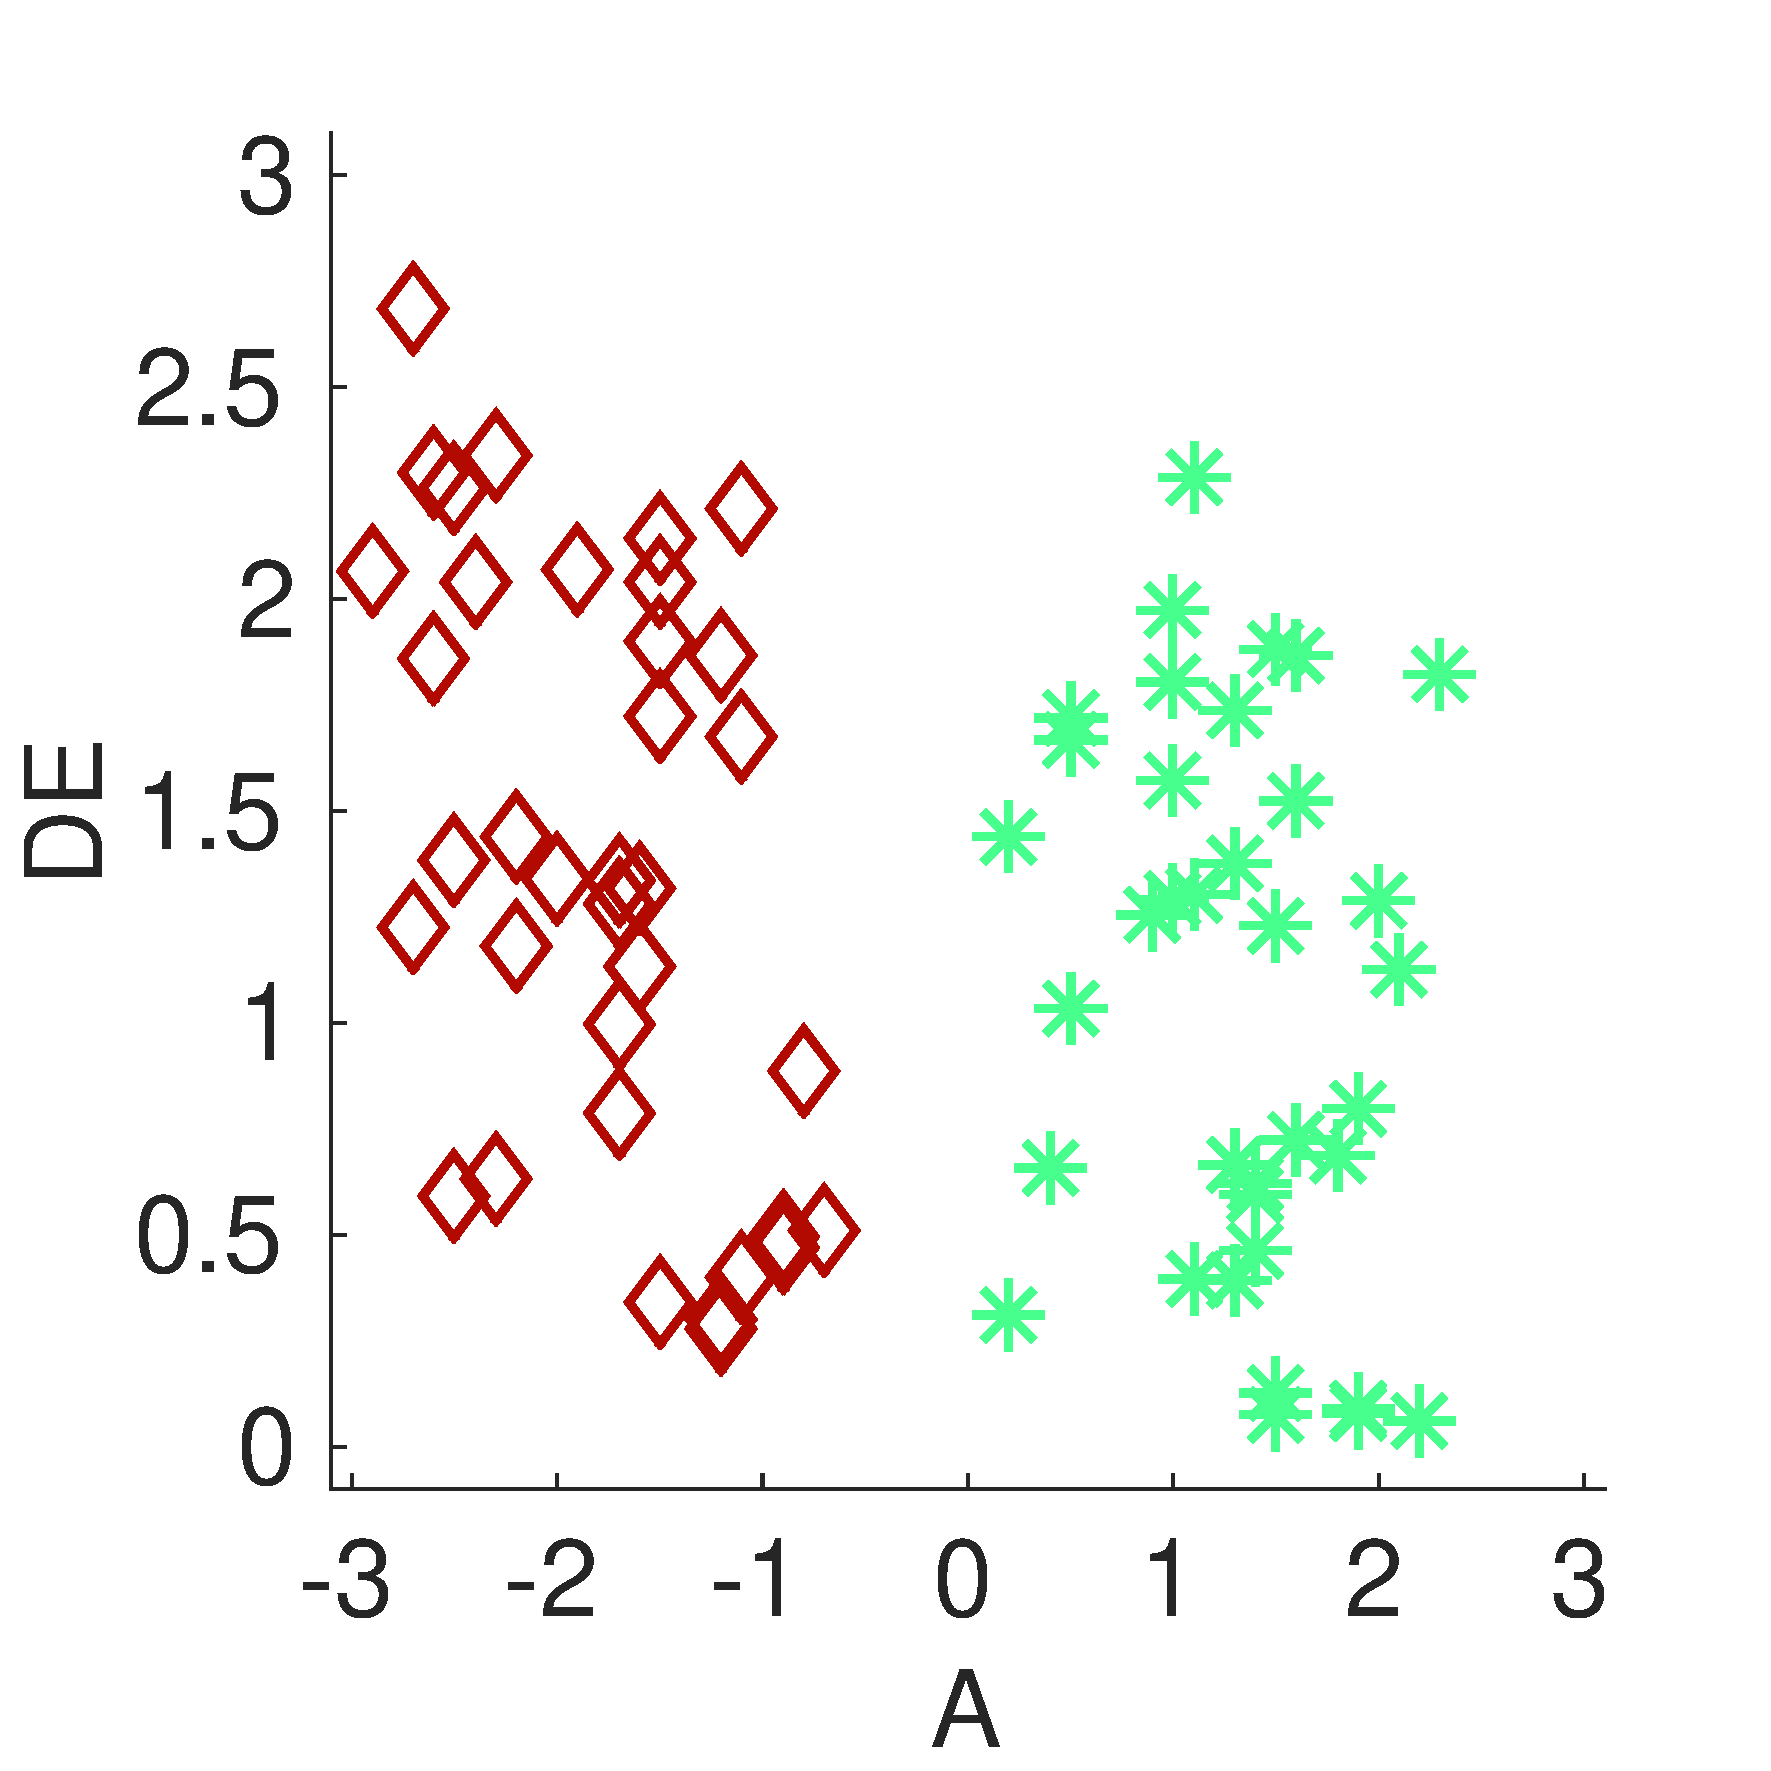
\includegraphics[width=.33\linewidth]{gfxXpUrbanSoundscape/xp_density_4}\label{fig:densityd}}
       \caption[TODO]{TODO}\label{fig:density}
\end{figure}

\subsection{Influence des descripteurs structurels sur l'agrément perçu}

Nous analysons maintenant l'existence de potentielles corrélations entre les descripteurs structurelles et $A$. Les coefficients de corrélation linéaire calculés entre $A$ \vs~$L$ et $D$ sont présentés dans le tableau~\ref{tab:corrStructA}.

\begin{table}[t]
\centering
\begin{tabular}{l c c c} 
            & ensemble                     & i-scènes                   & ni-scènes    \\
\hline
$L$         & \textbf{-0.76} ($p<0.01$)    & -0.32 ($p=0.06$)           & \textbf{-0.67} ($p<0.01$)\\
$LE$        & \textbf{-0.75} ($p<0.01$)    & -0.20 ($p=0.24$)           & \textbf{-0.75} ($p<0.01$)\\
$LT$        & \textbf{-0.51} ($p<0.01$)    & -0.33 ($p=0.05$)           &  0.09  ($p=0.6$) \\
$D$         & \textbf{-0.41} ($p<0.01$)    & -0.31 ($p=0.07$)           & -0.37 ($p=0.03$)\\
$DE$        & \textbf{-0.34} ($p<0.01$)    & -0.22 ($p=0.21$)           & \textbf{-0.47} ($p<0.01$)\\
\hline
\end{tabular}
\vspace{0.5mm}
\caption{Coefficients de corrélation linéaire calculés entre l'agrément perçu moyen $A$ \vs~TODO}
\label{tab:corrStructA}
\end{table}

\begin{figure}[bth]
        \myfloatalign
        \includegraphics[width=.9\linewidth]{gfxXpUrbanSoundscape/xp1_div_1}
       \caption[TODO]{TODO}\label{fig:diversity}
\end{figure}

\subsection{Étude comparative entre les descripteurs sémantiques}

\begin{table}[t]
 \setlength{\tabcolsep}{0.2pt}
 \centering
  {\renewcommand{\arraystretch}{0.9}
\begin{tabular}{c c c c} 
Niveau        & \multicolumn{2}{c}{Marqueurs sonores} \\
d'abstraction & i-scènes & ni-scènes \\
\hline
0  &                               &  construction work (3.78)  \\
\hline
  & church bell  (4.5)             & horn  (3.9) \\
1 & bell bike    (4.3)             & siren (3.9)\\
  & animal       (4.2)             &       \\
   \hline
  & birds        (4.8)             & horn  (4.0)\\
2 & church bell  (4.4)             & siren (4.0)\\
  & bell bike    (4.2)             &       \\
   \hline
  & birds singing (4.8)            & horn  (4.1)\\
  & church bell   (4.3)            & siren (4.0)\\
3 & bell bike     (4.2)            &       \\
  & male footsteps                 &  \\
  &   concrete (3.6)               &  \\
  \hline
\end{tabular}
}
\vspace{0.5mm}
\caption[Classes d'événements identifiées comme étant des marqueurs sonores]{Classes d'événements identifiées comme étant des marqueurs sonores. Dans chaque cellule, les marqueurs sont ordonnés par ordre décroissant de valeur $V$.}
\label{tab:markers}
\end{table}

\subsection{Étude des espaces de représentations induits par les descripteurs sémantiques}

\begin{figure}[bth]
        \myfloatalign
        \includegraphics[width=.9\linewidth]{gfxXpUrbanSoundscape/pa5_1}
       \caption[TODO]{TODO}\label{fig:pa5}
\end{figure}

\subsection{L'influence spécifique des marqueurs sonores sur l'agrément perçu}

\begin{table}[t]
\centering
\begin{tabular}{l r r} 
               &   i-scenes                   & ni-scenes \\
\hline
$L_m$            & 0.03  ($p=0.88$)           & \textbf{-0.63} ($p<0.01$) \\
$LE_m$           & 0.08  ($p=0.66$)           & \textbf{-0.60} ($p<0.01$) \\
$LT_m$           & -0.11 ($p=0.66$)           & -0.00 ($p=0.98$) \\
$D_m$            & 0.03 ($p=0.85$)            & -0.32 ($p=0.05$) \\
$DE_m$           & 0.09  ($p=0.62$)           & \textbf{-0.47} ($p<0.01$) \\
$L_m-L_b$        & \textbf{0.67} ($p<0.01$)   & -0.24 ($p=0.15$) \\
$LE_m-LE_b$      & \textbf{0.66} ($p<0.01$)   & -0.31 ($p=0.06$) \\
$LT_m-LT_b$      & 0.16 ($p=0.54$)            &  0.39 ($p<0.05$) \\

\hline
\end{tabular}
\vspace{0.5mm}
\caption{Coefficients de corrélation linéaire calculés entre l'agrément perçu moyen $A$ \vs~TODO.}
\label{tab:coorMarkers}
\end{table}

\begin{figure}[bth]
        \myfloatalign
        \subfloat[]
        {\includegraphics[width=.33\linewidth]{gfxXpUrbanSoundscape/xp_soundlevel_7}\label{fig:soundlevelMarkera}}
        \subfloat[]
        {\includegraphics[width=.33\linewidth]{gfxXpUrbanSoundscape/xp_soundlevel_11}\label{fig:soundlevelMarkerb}}
        \subfloat[]
        {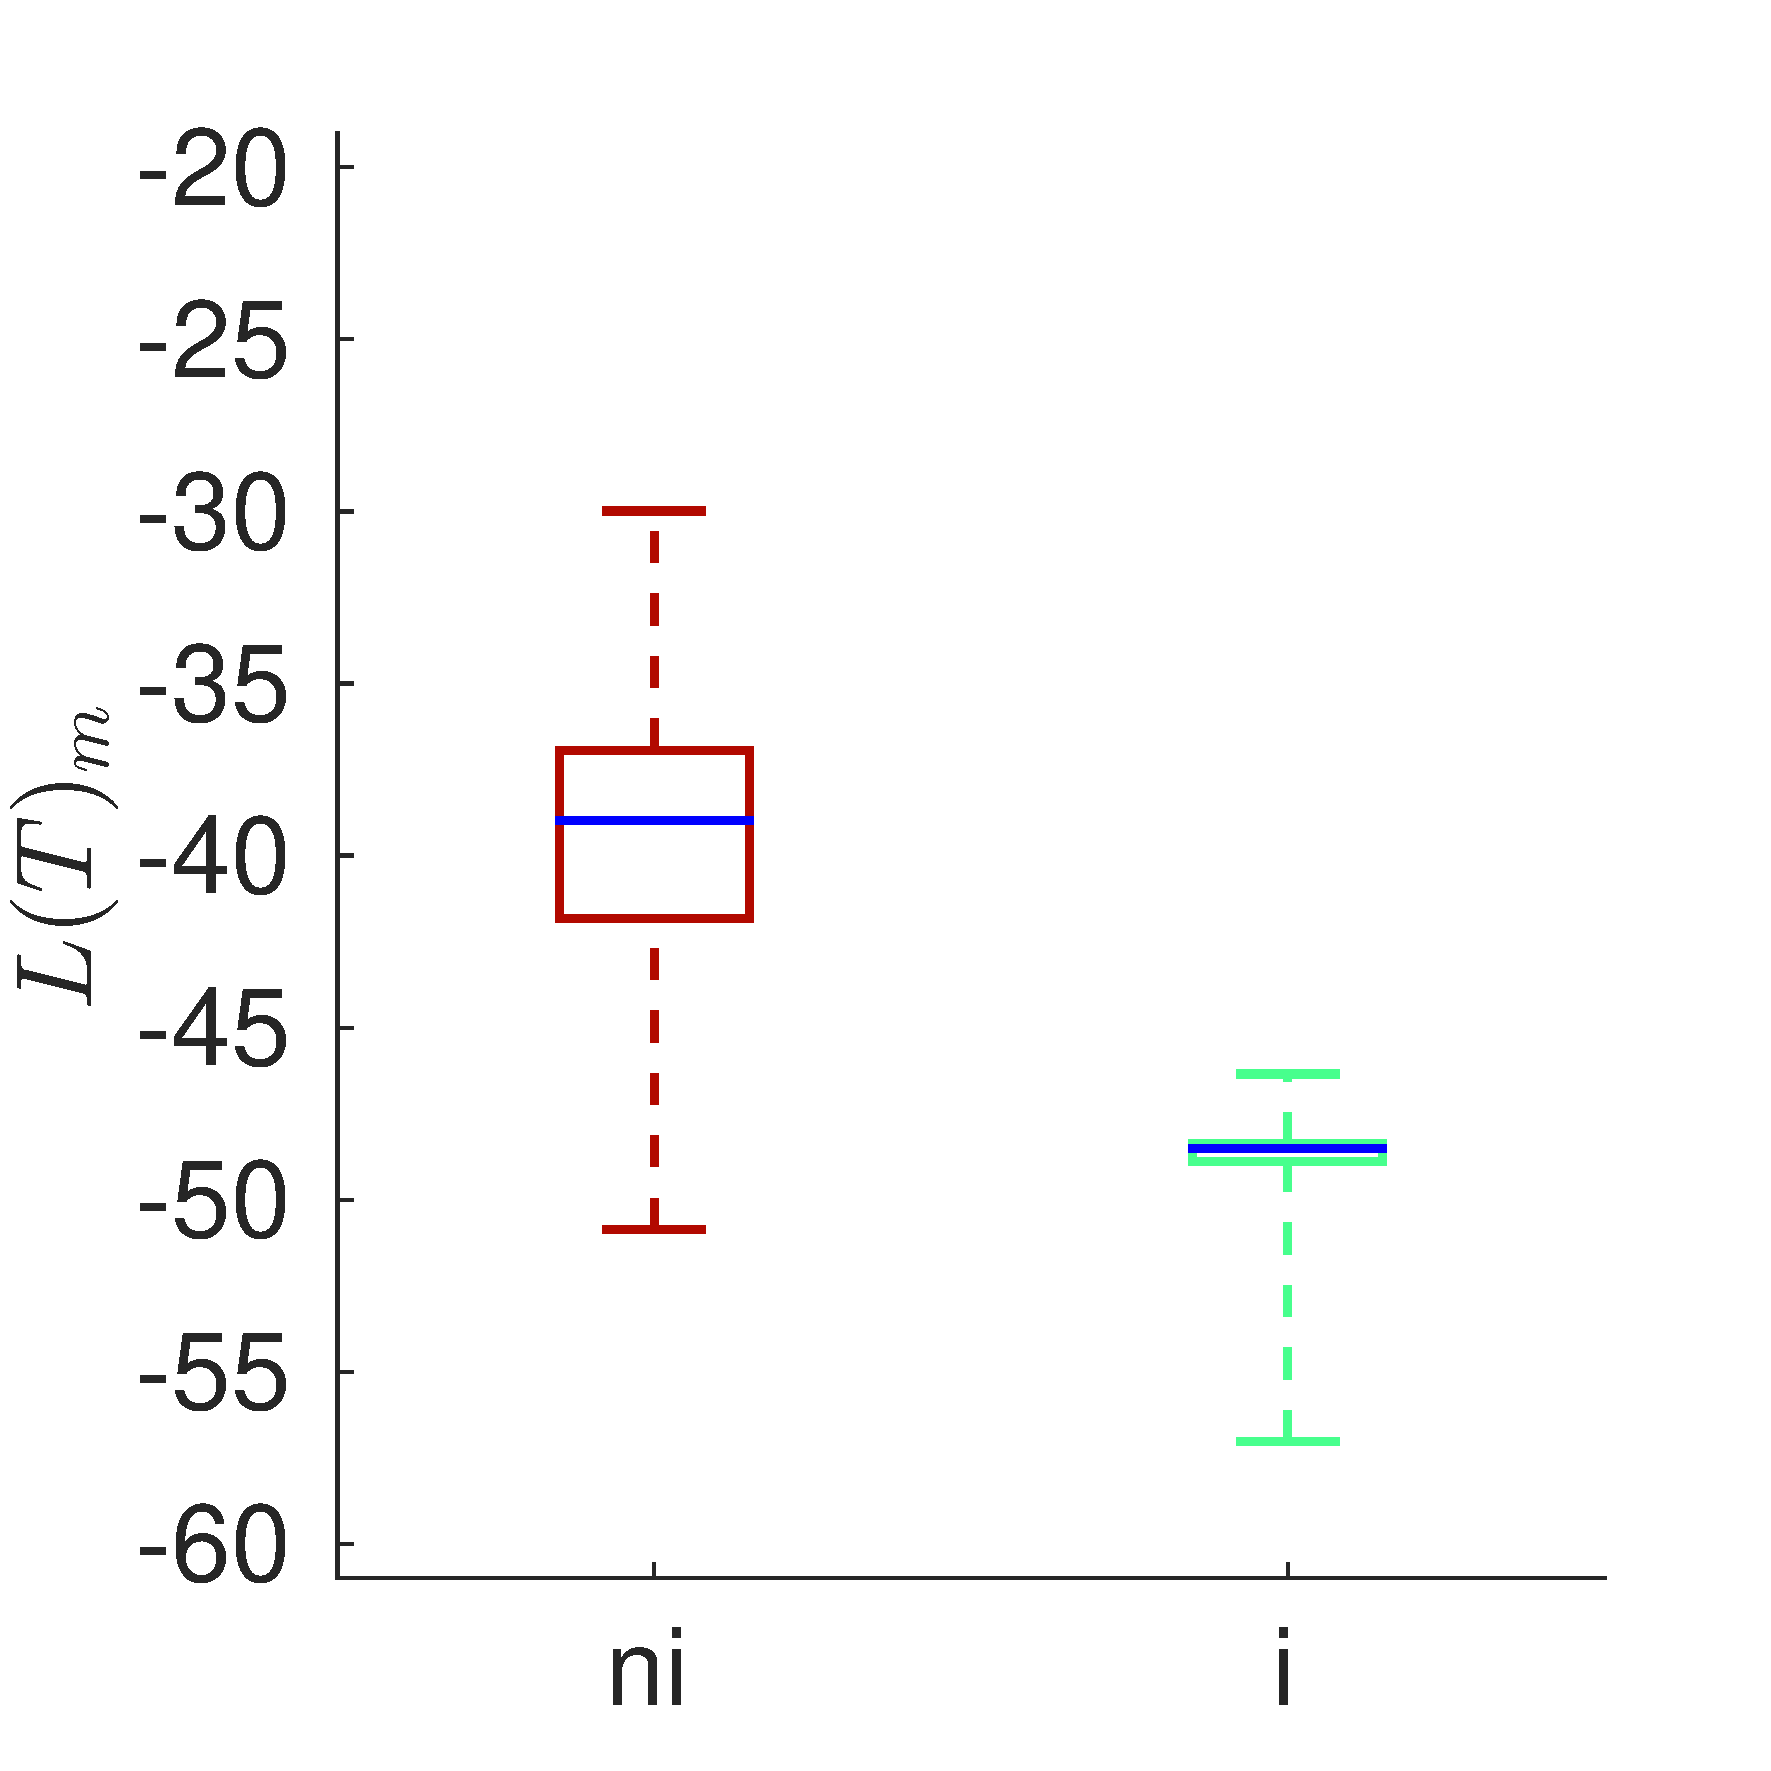
\includegraphics[width=.33\linewidth]{gfxXpUrbanSoundscape/xp_soundlevel_15}\label{fig:soundlevelMarkerc}}\par
        \subfloat[]
        {\includegraphics[width=.33\linewidth]{gfxXpUrbanSoundscape/xp_soundlevel_8}\label{fig:soundlevelMarkerd}}
        \subfloat[]
        {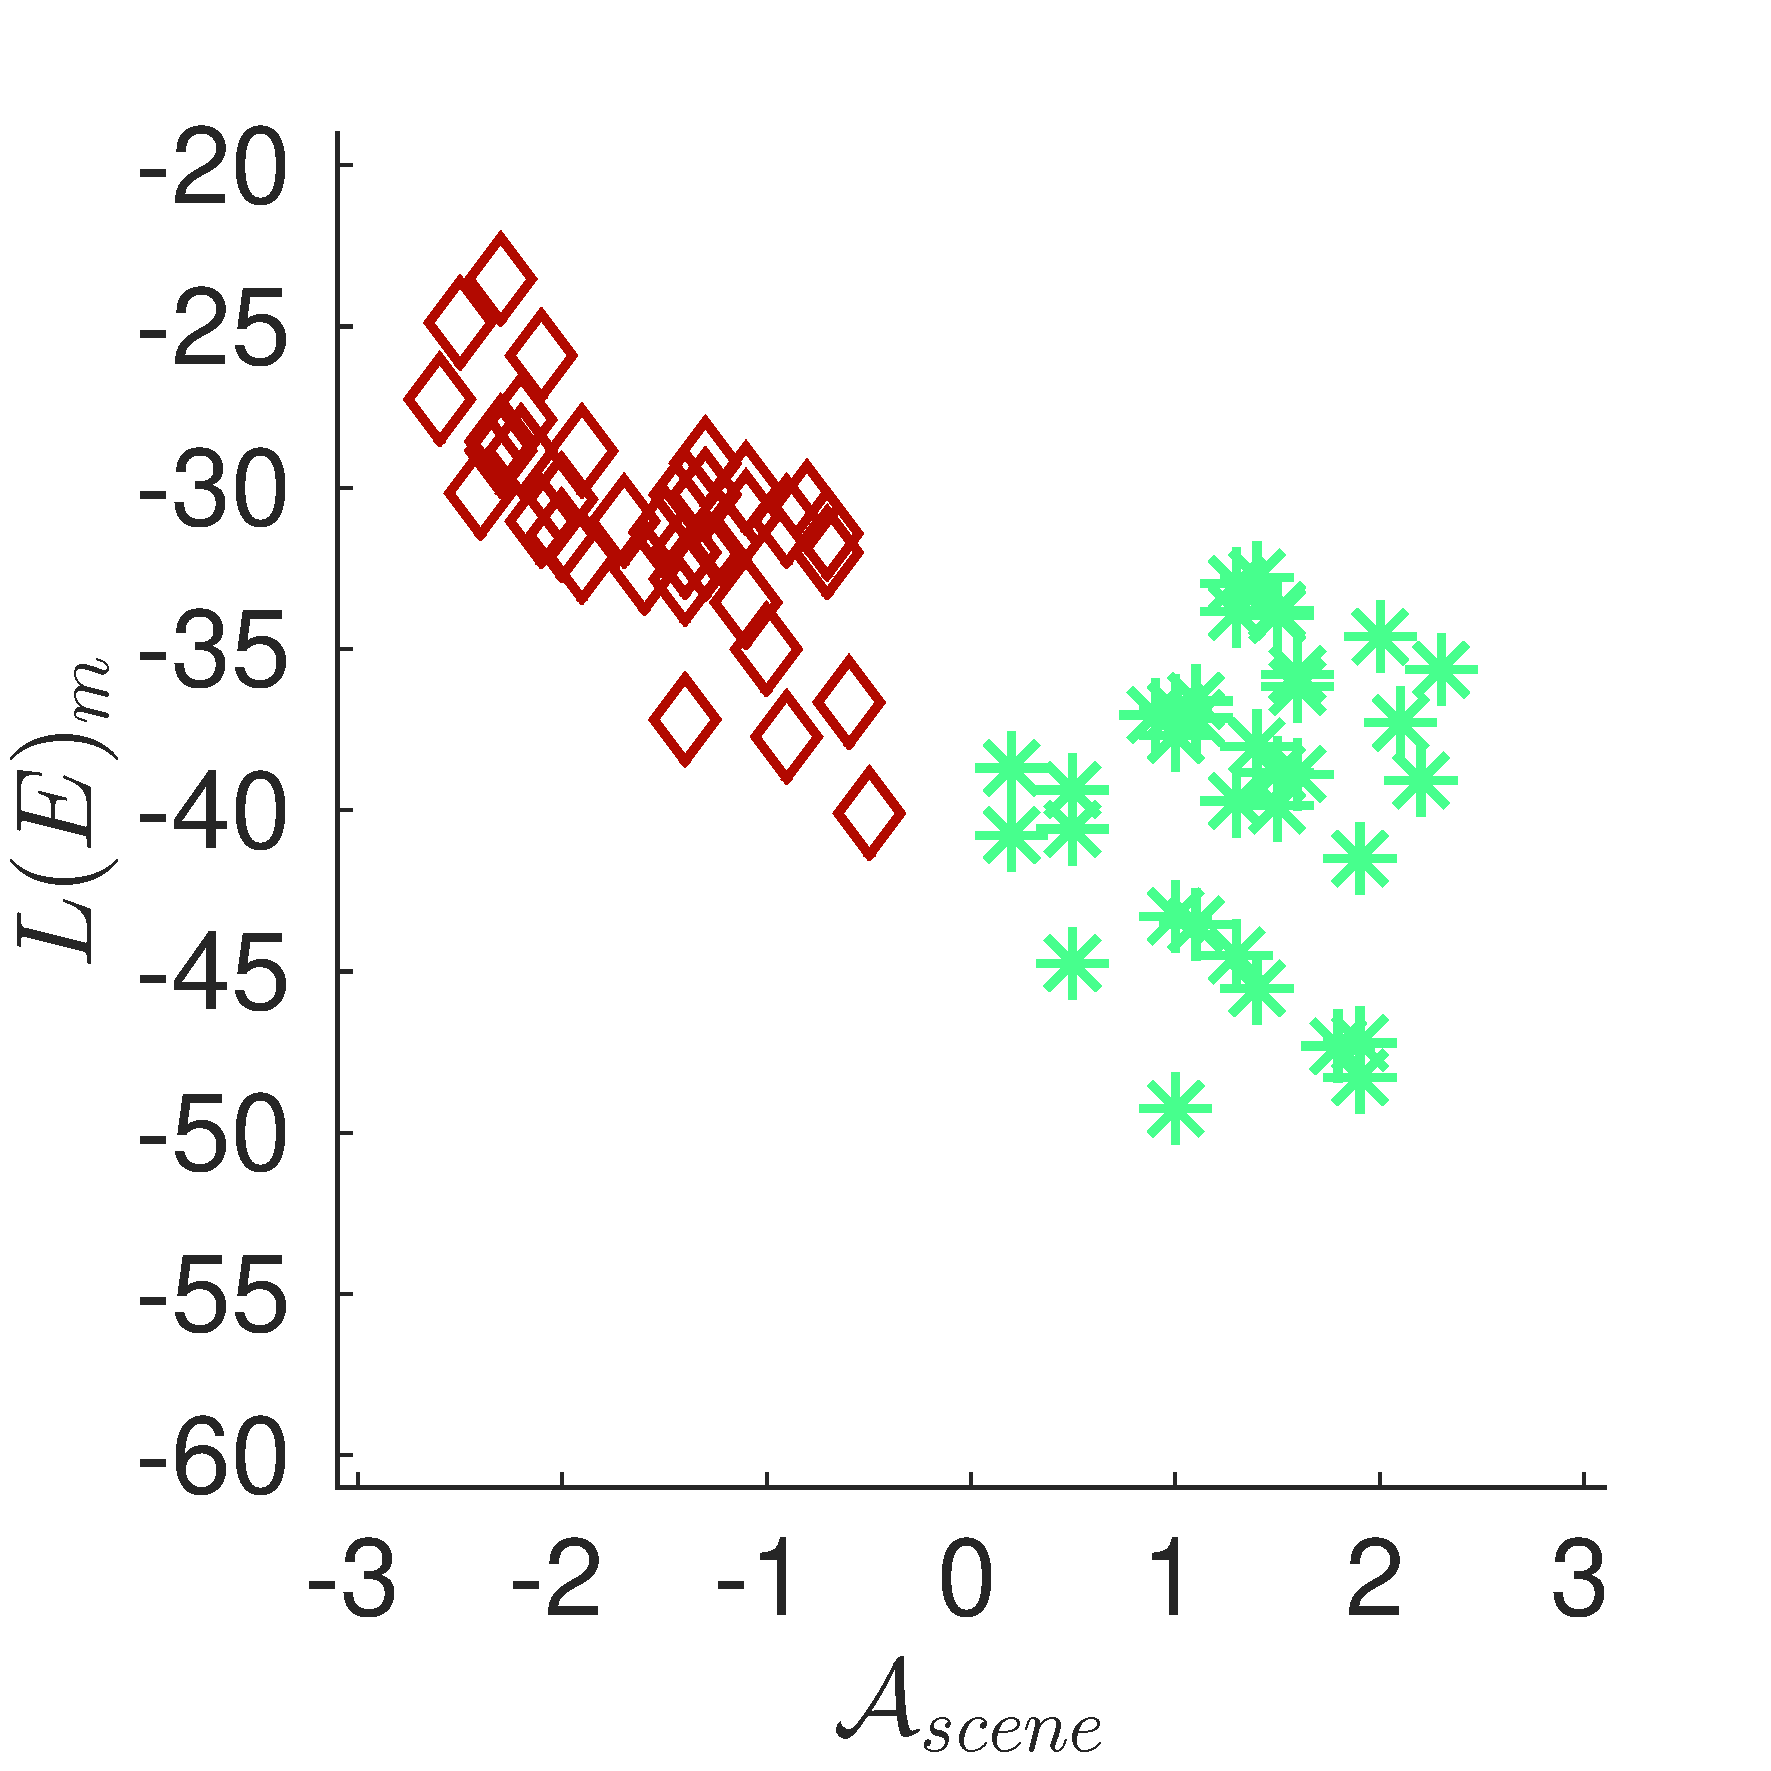
\includegraphics[width=.33\linewidth]{gfxXpUrbanSoundscape/xp_soundlevel_12}\label{fig:soundlevelMarkere}}
        \subfloat[]
        {\includegraphics[width=.33\linewidth]{gfxXpUrbanSoundscape/xp_soundlevel_16}\label{fig:soundlevelMarkerf}}
       \caption[TODO]{TODO}\label{fig:soundlevelMarker}
\end{figure}

\begin{figure}[bth]
        \myfloatalign
        \subfloat[]
        {\includegraphics[width=.33\linewidth]{gfxXpUrbanSoundscape/xp_density_7}\label{fig:densityMarkera}}
        \subfloat[]
        {\includegraphics[width=.33\linewidth]{gfxXpUrbanSoundscape/xp_density_9}\label{fig:densityMarkerb}}\par
        \subfloat[]
        {\includegraphics[width=.33\linewidth]{gfxXpUrbanSoundscape/xp_density_8}\label{fig:densityMarkerc}}
        \subfloat[]
        {\includegraphics[width=.33\linewidth]{gfxXpUrbanSoundscape/xp_density_10}\label{fig:densityMarkerd}}
       \caption[TODO]{TODO}\label{fig:densityMarker}
\end{figure}

\begin{figure}[bth]
        \myfloatalign
        \subfloat[]
        {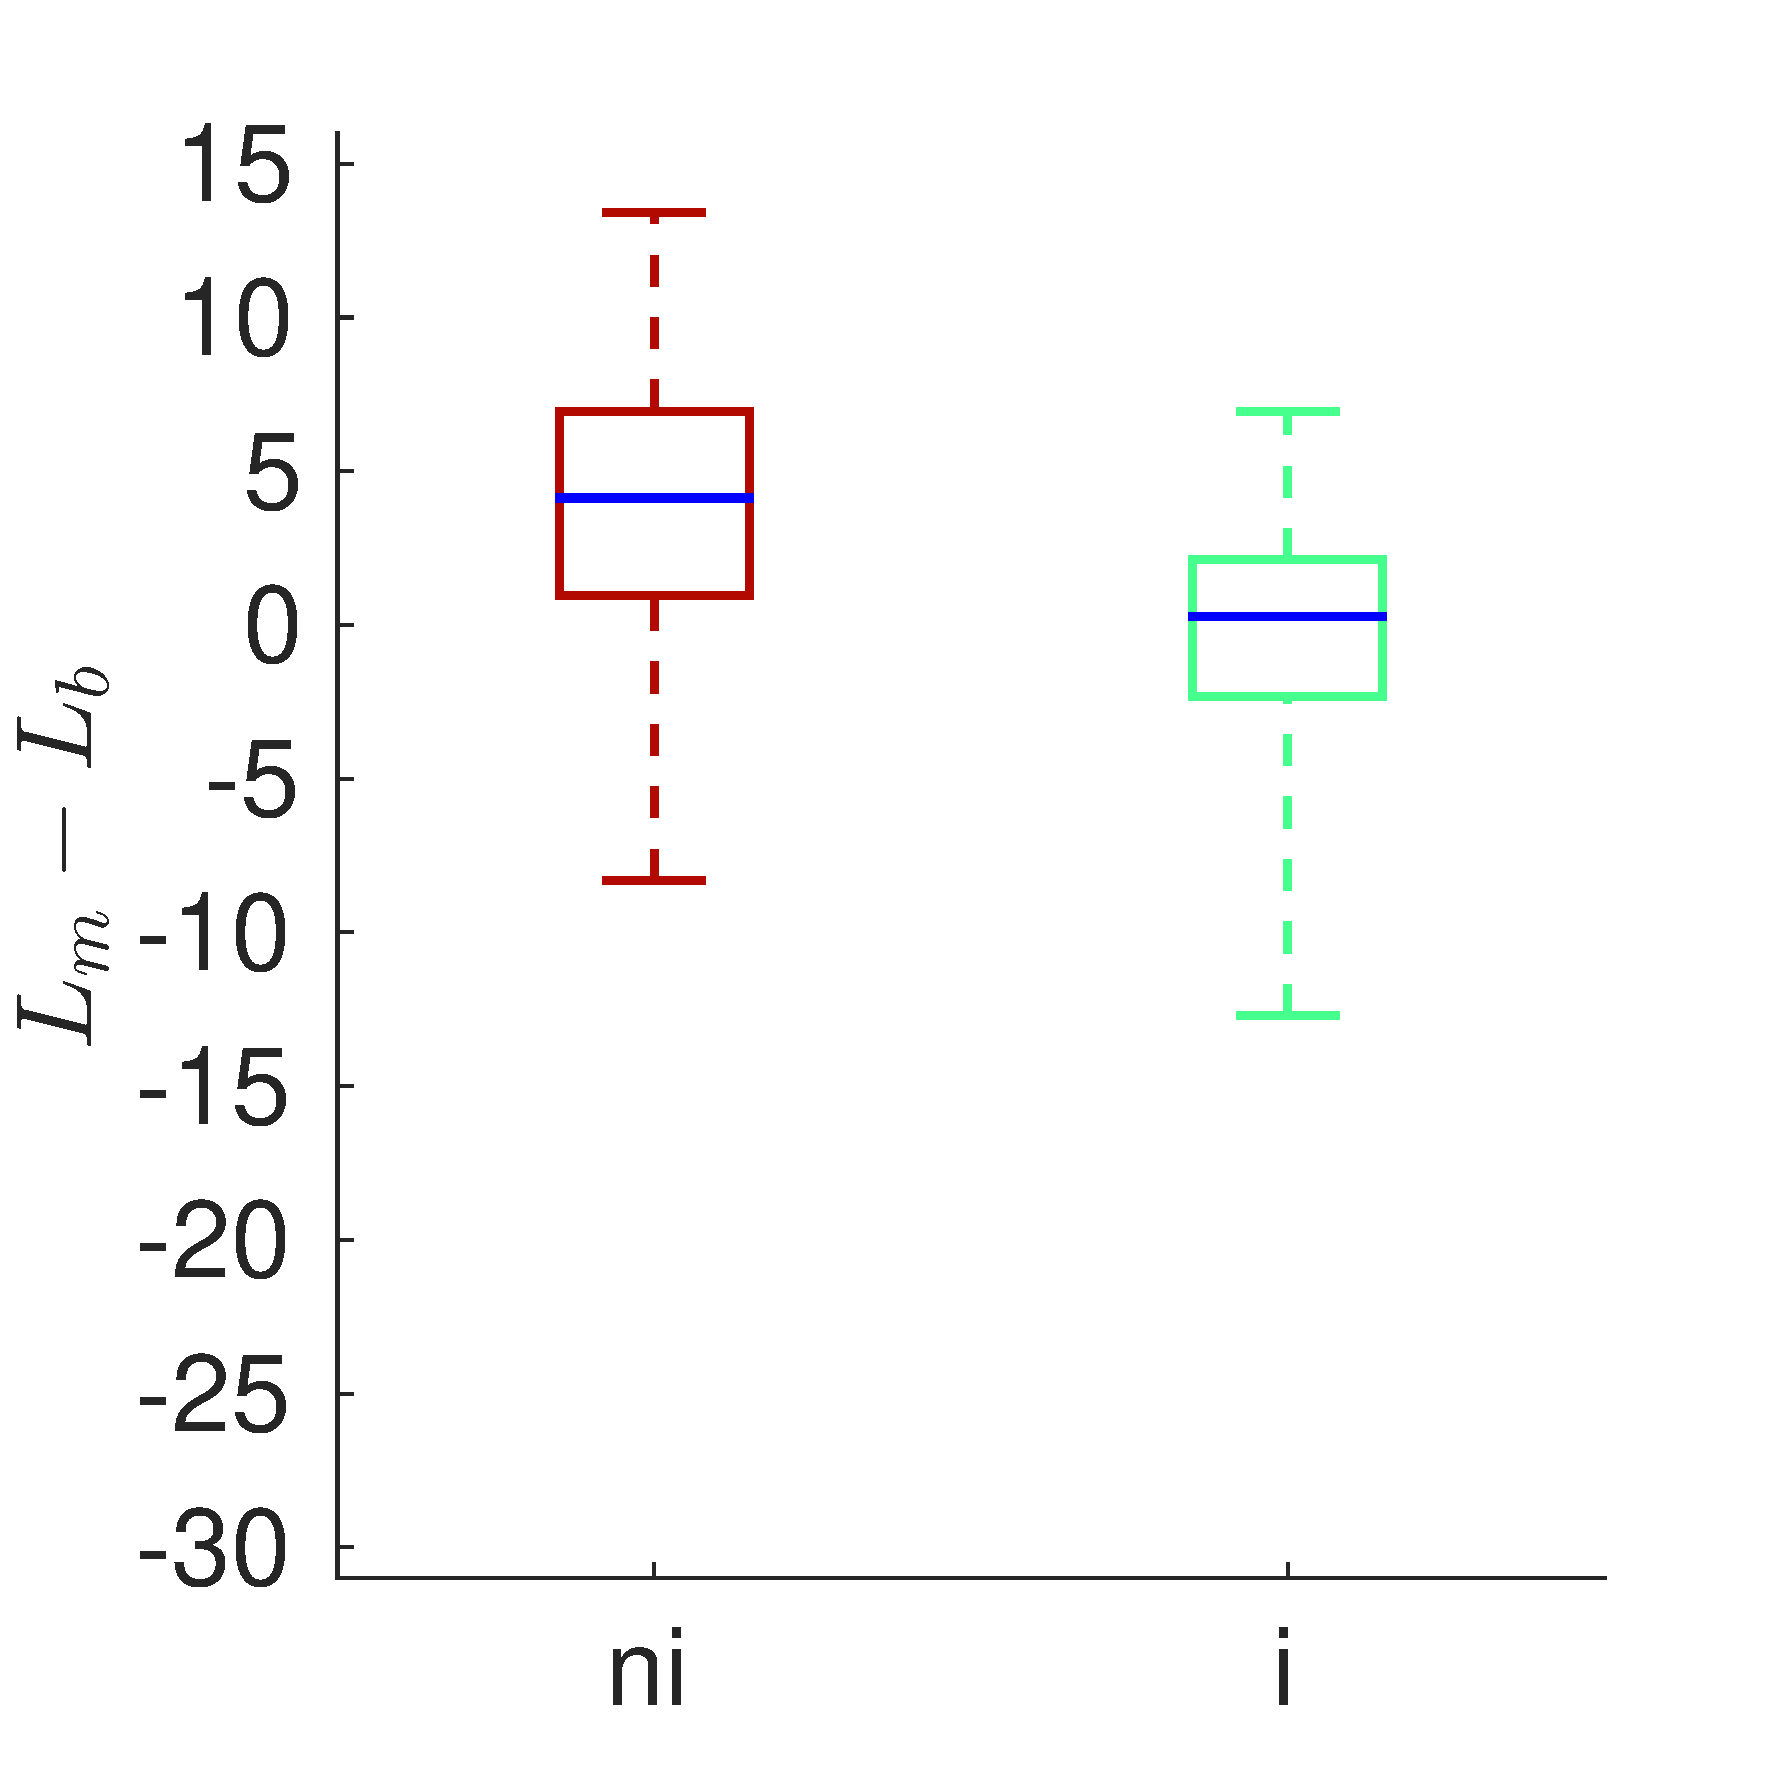
\includegraphics[width=.33\linewidth]{gfxXpUrbanSoundscape/xp_soundlevel_19}\label{fig:soundlevelMarkerDiffa}}
        \subfloat[]
        {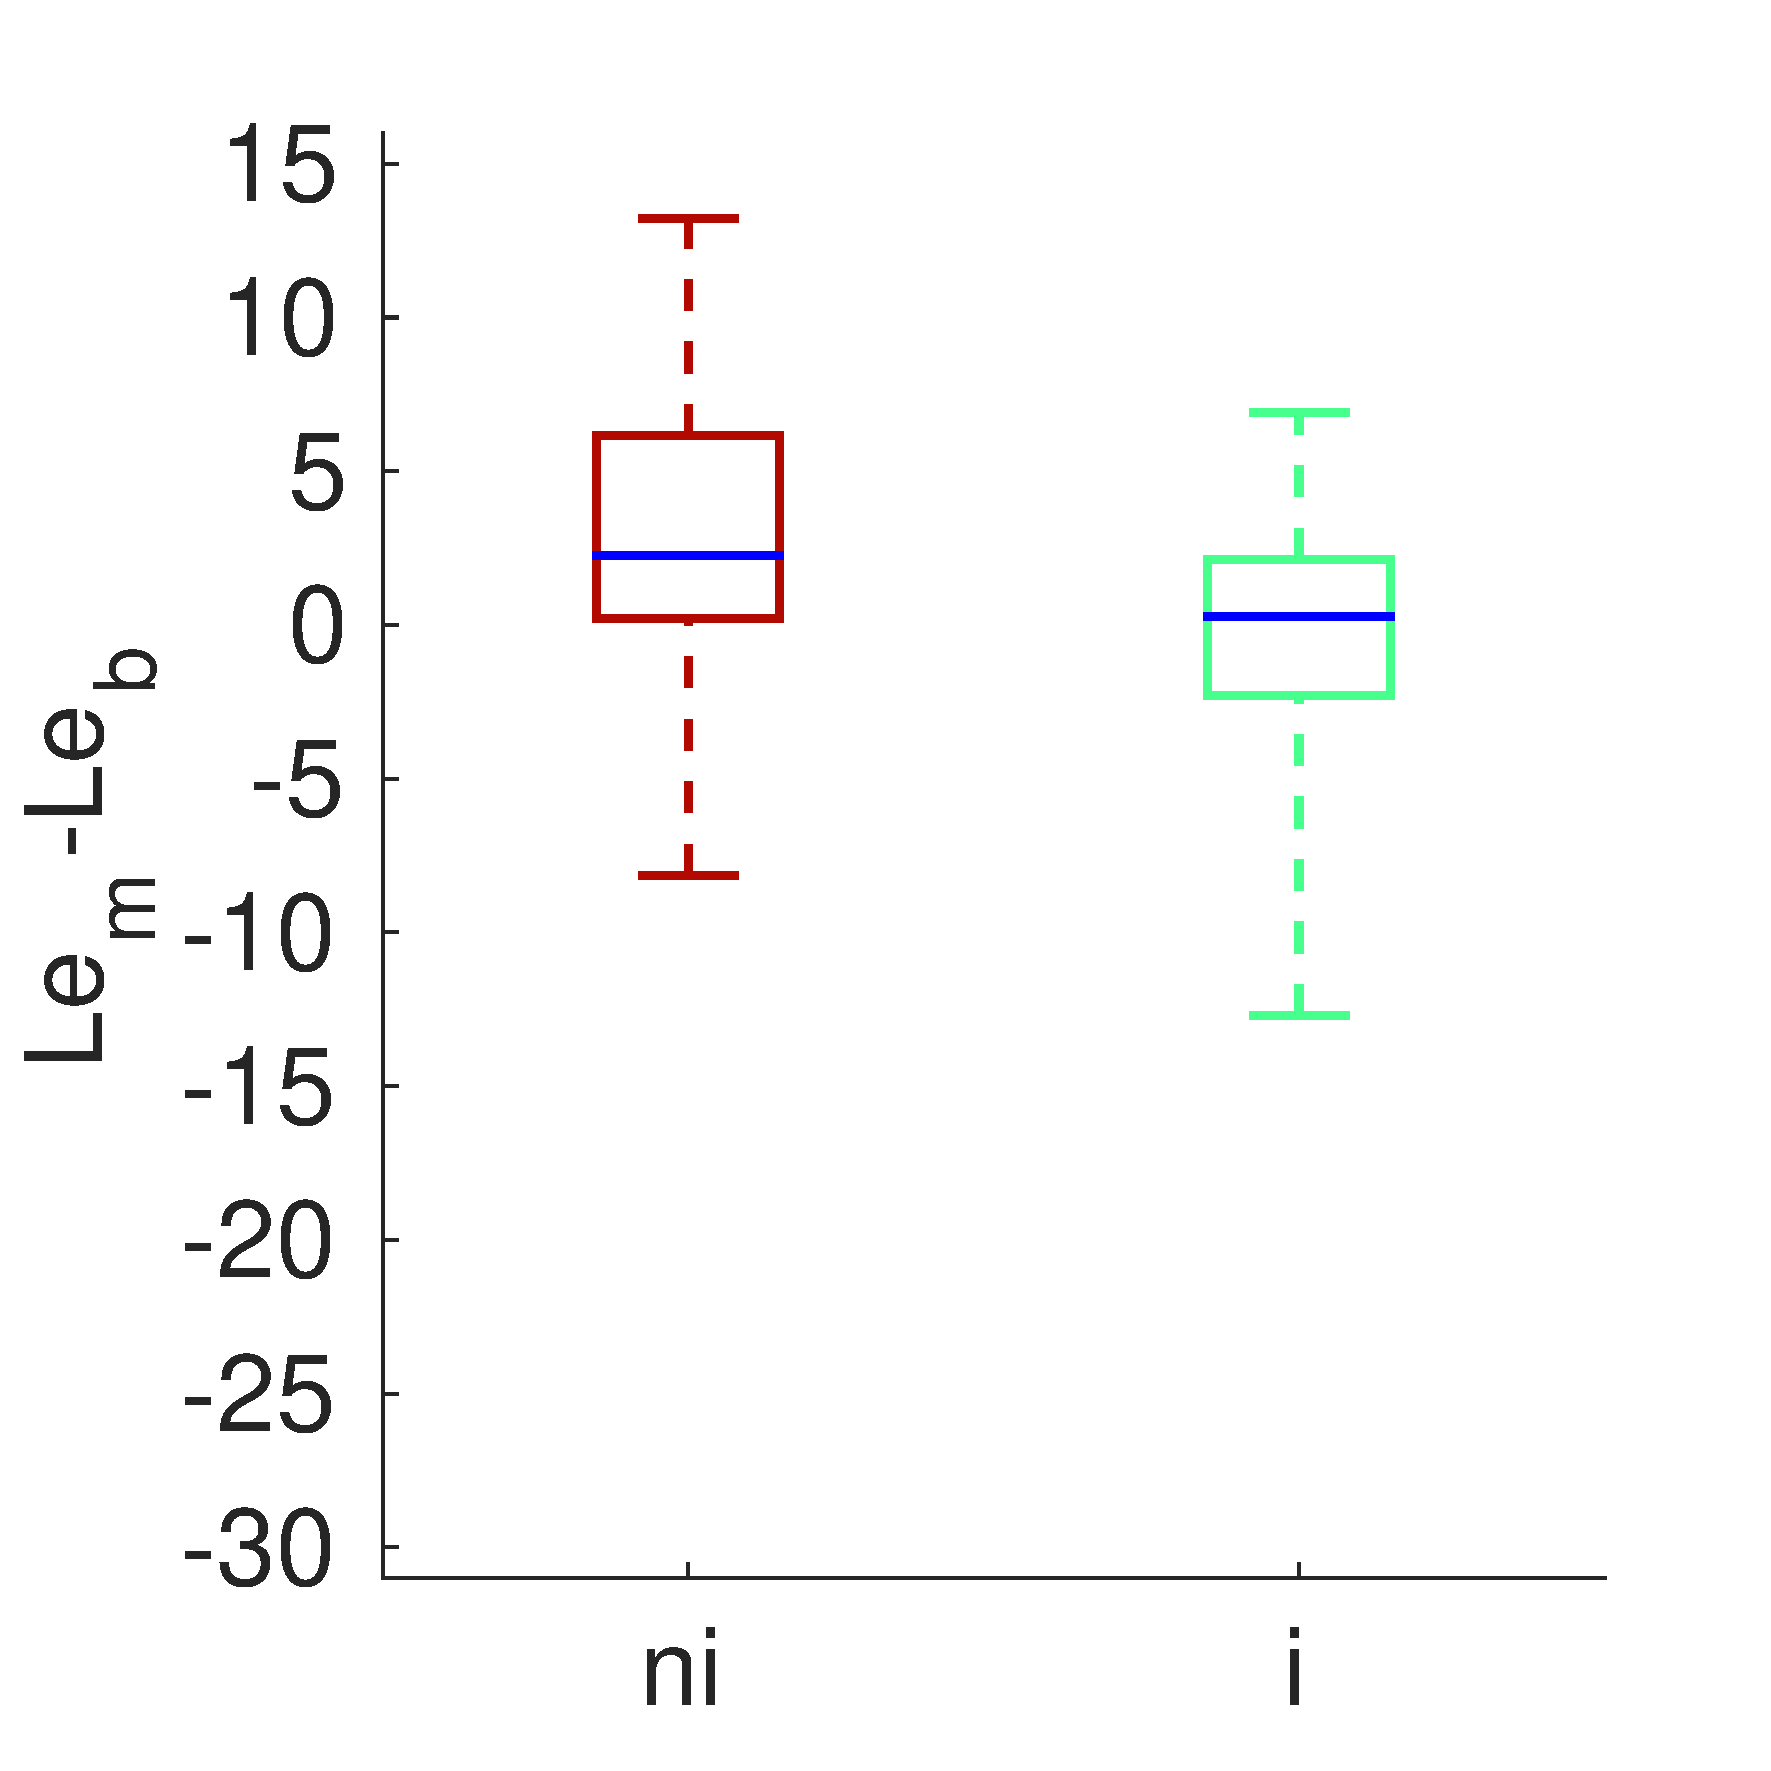
\includegraphics[width=.33\linewidth]{gfxXpUrbanSoundscape/xp_soundlevel_21}\label{fig:soundlevelMarkerDiffb}}
        \subfloat[]
        {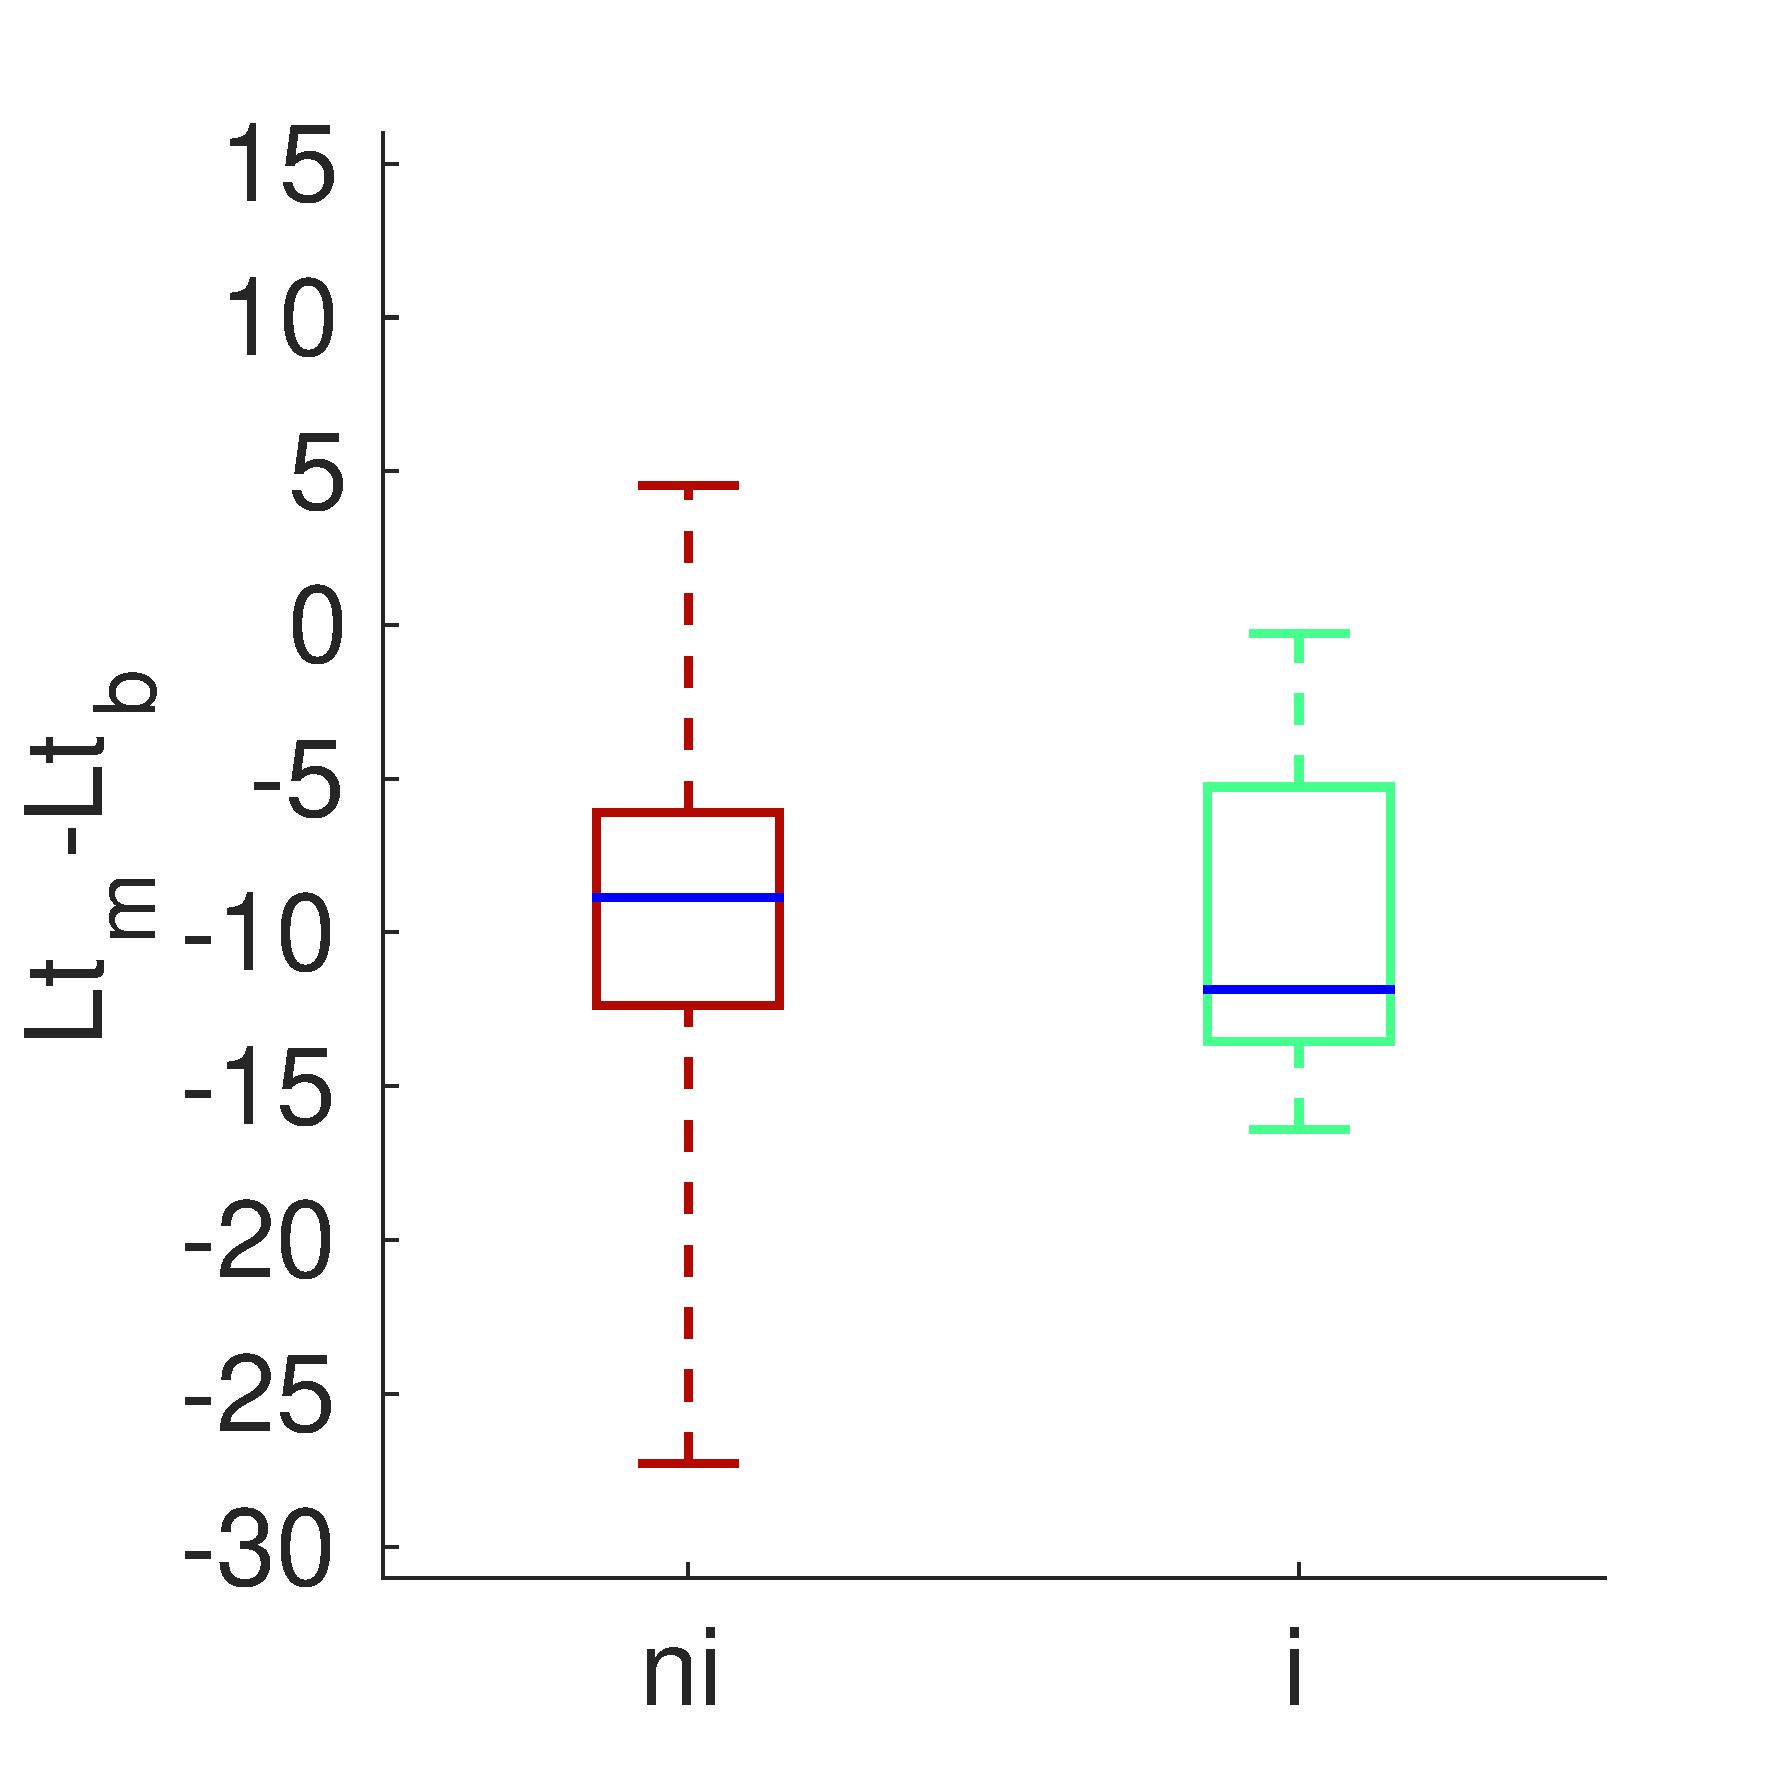
\includegraphics[width=.33\linewidth]{gfxXpUrbanSoundscape/xp_soundlevel_23}\label{fig:soundlevelMarkerDiffc}}\par
        \subfloat[]
        {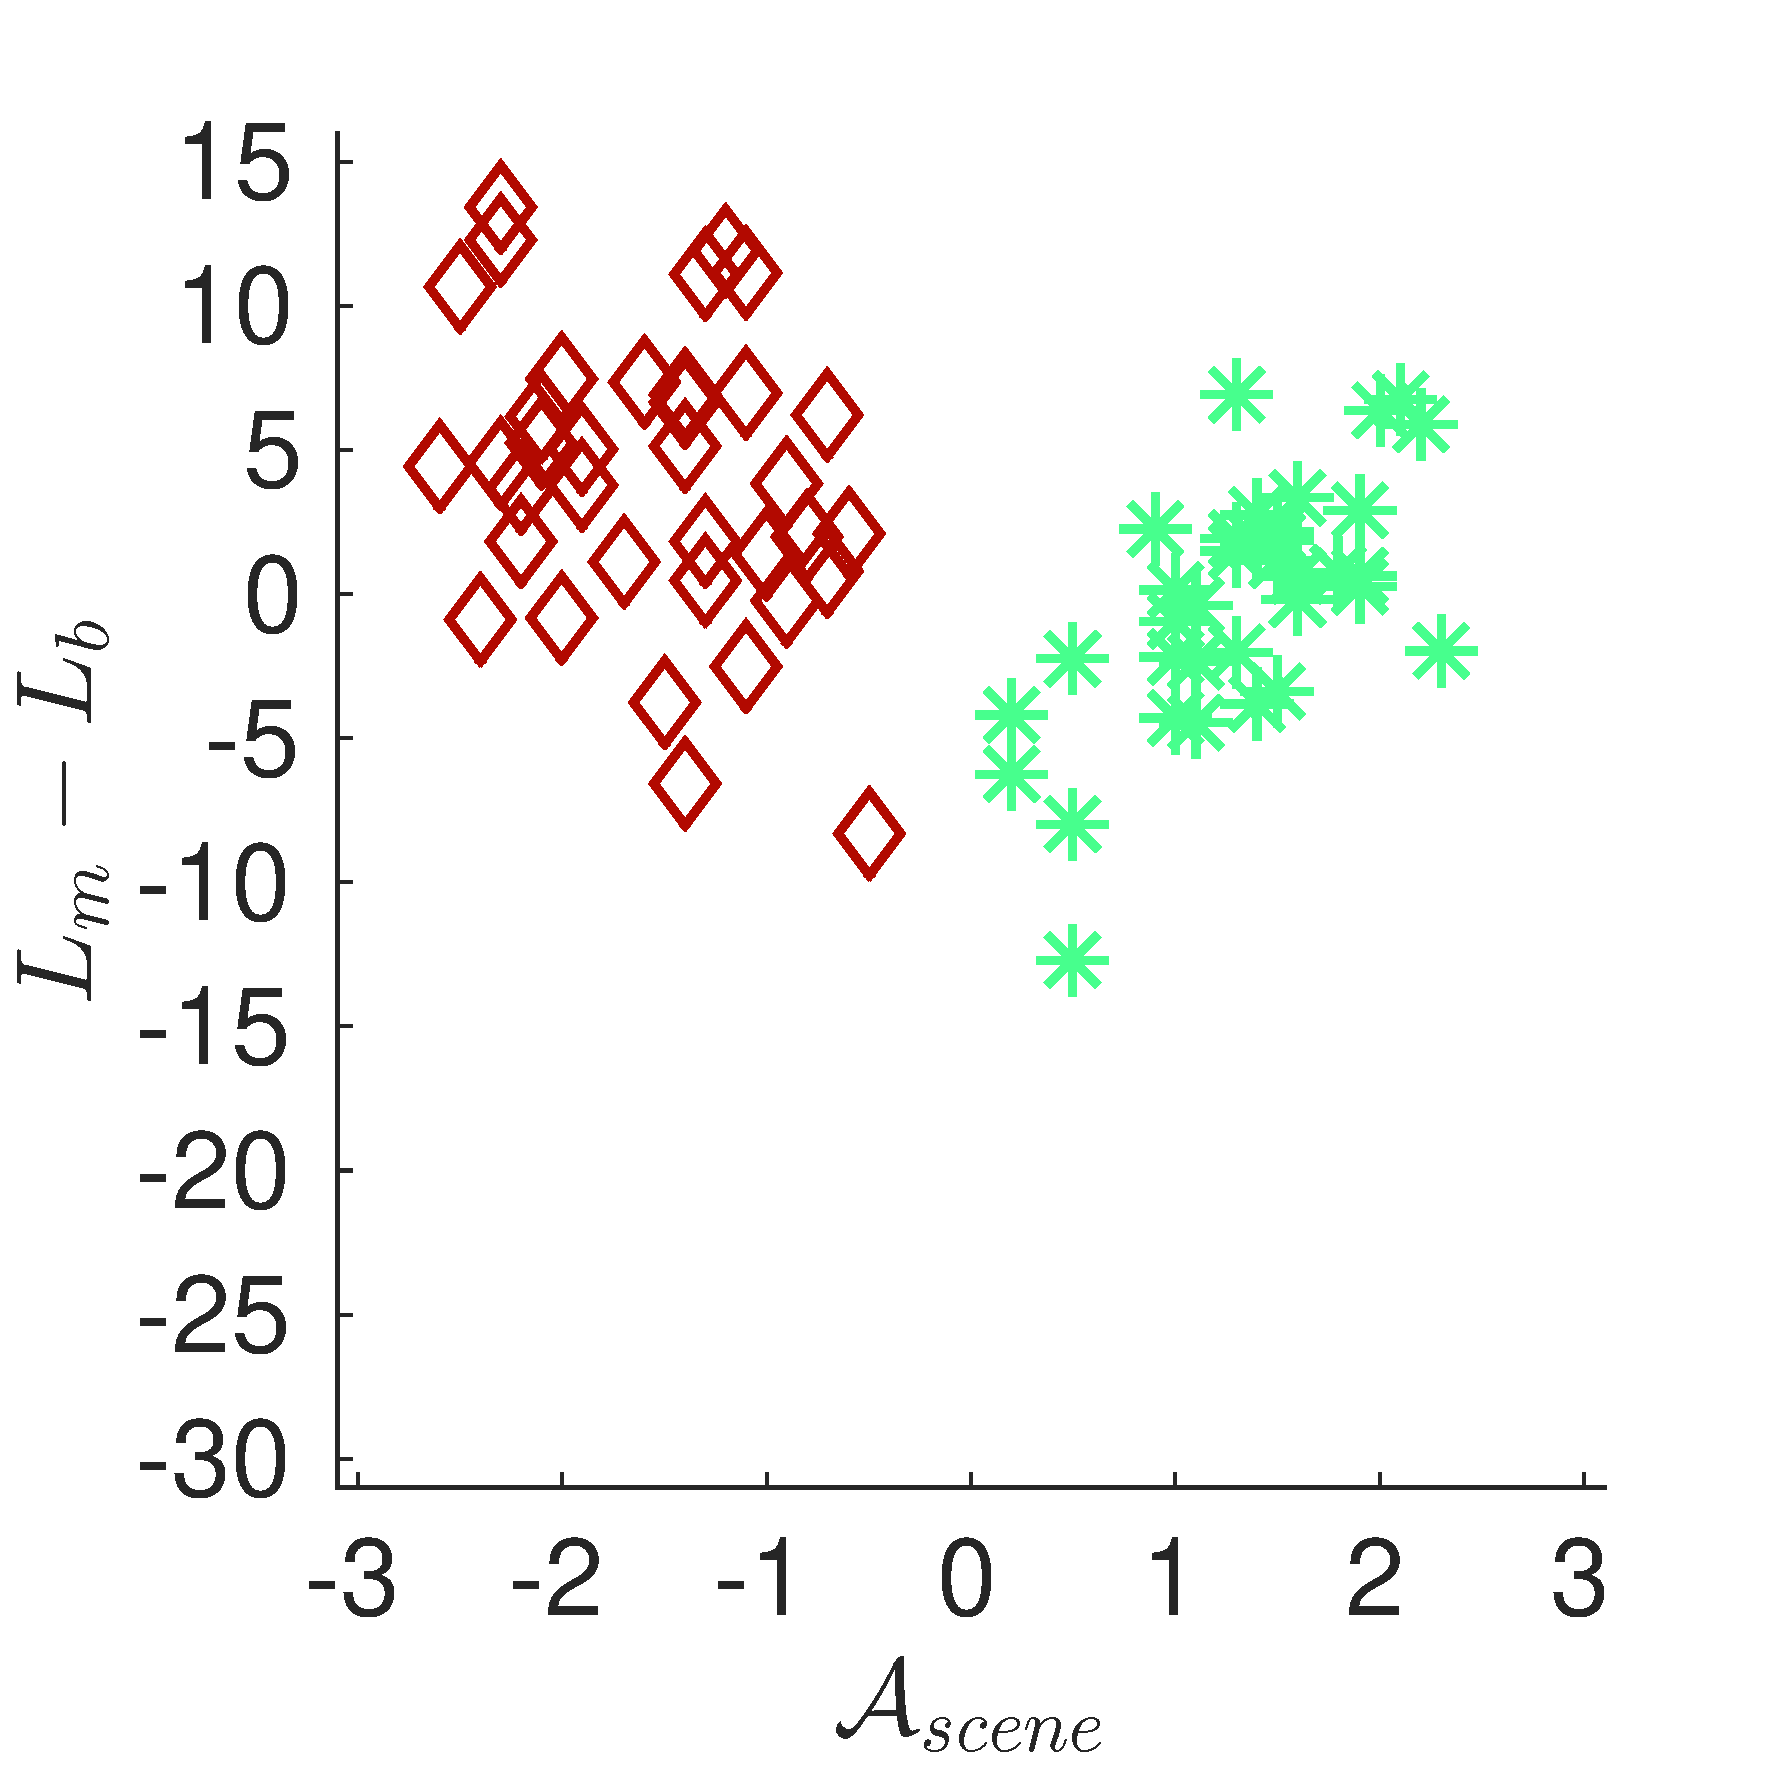
\includegraphics[width=.33\linewidth]{gfxXpUrbanSoundscape/xp_soundlevel_20}\label{fig:soundlevelMarkerDiffd}}
        \subfloat[]
        {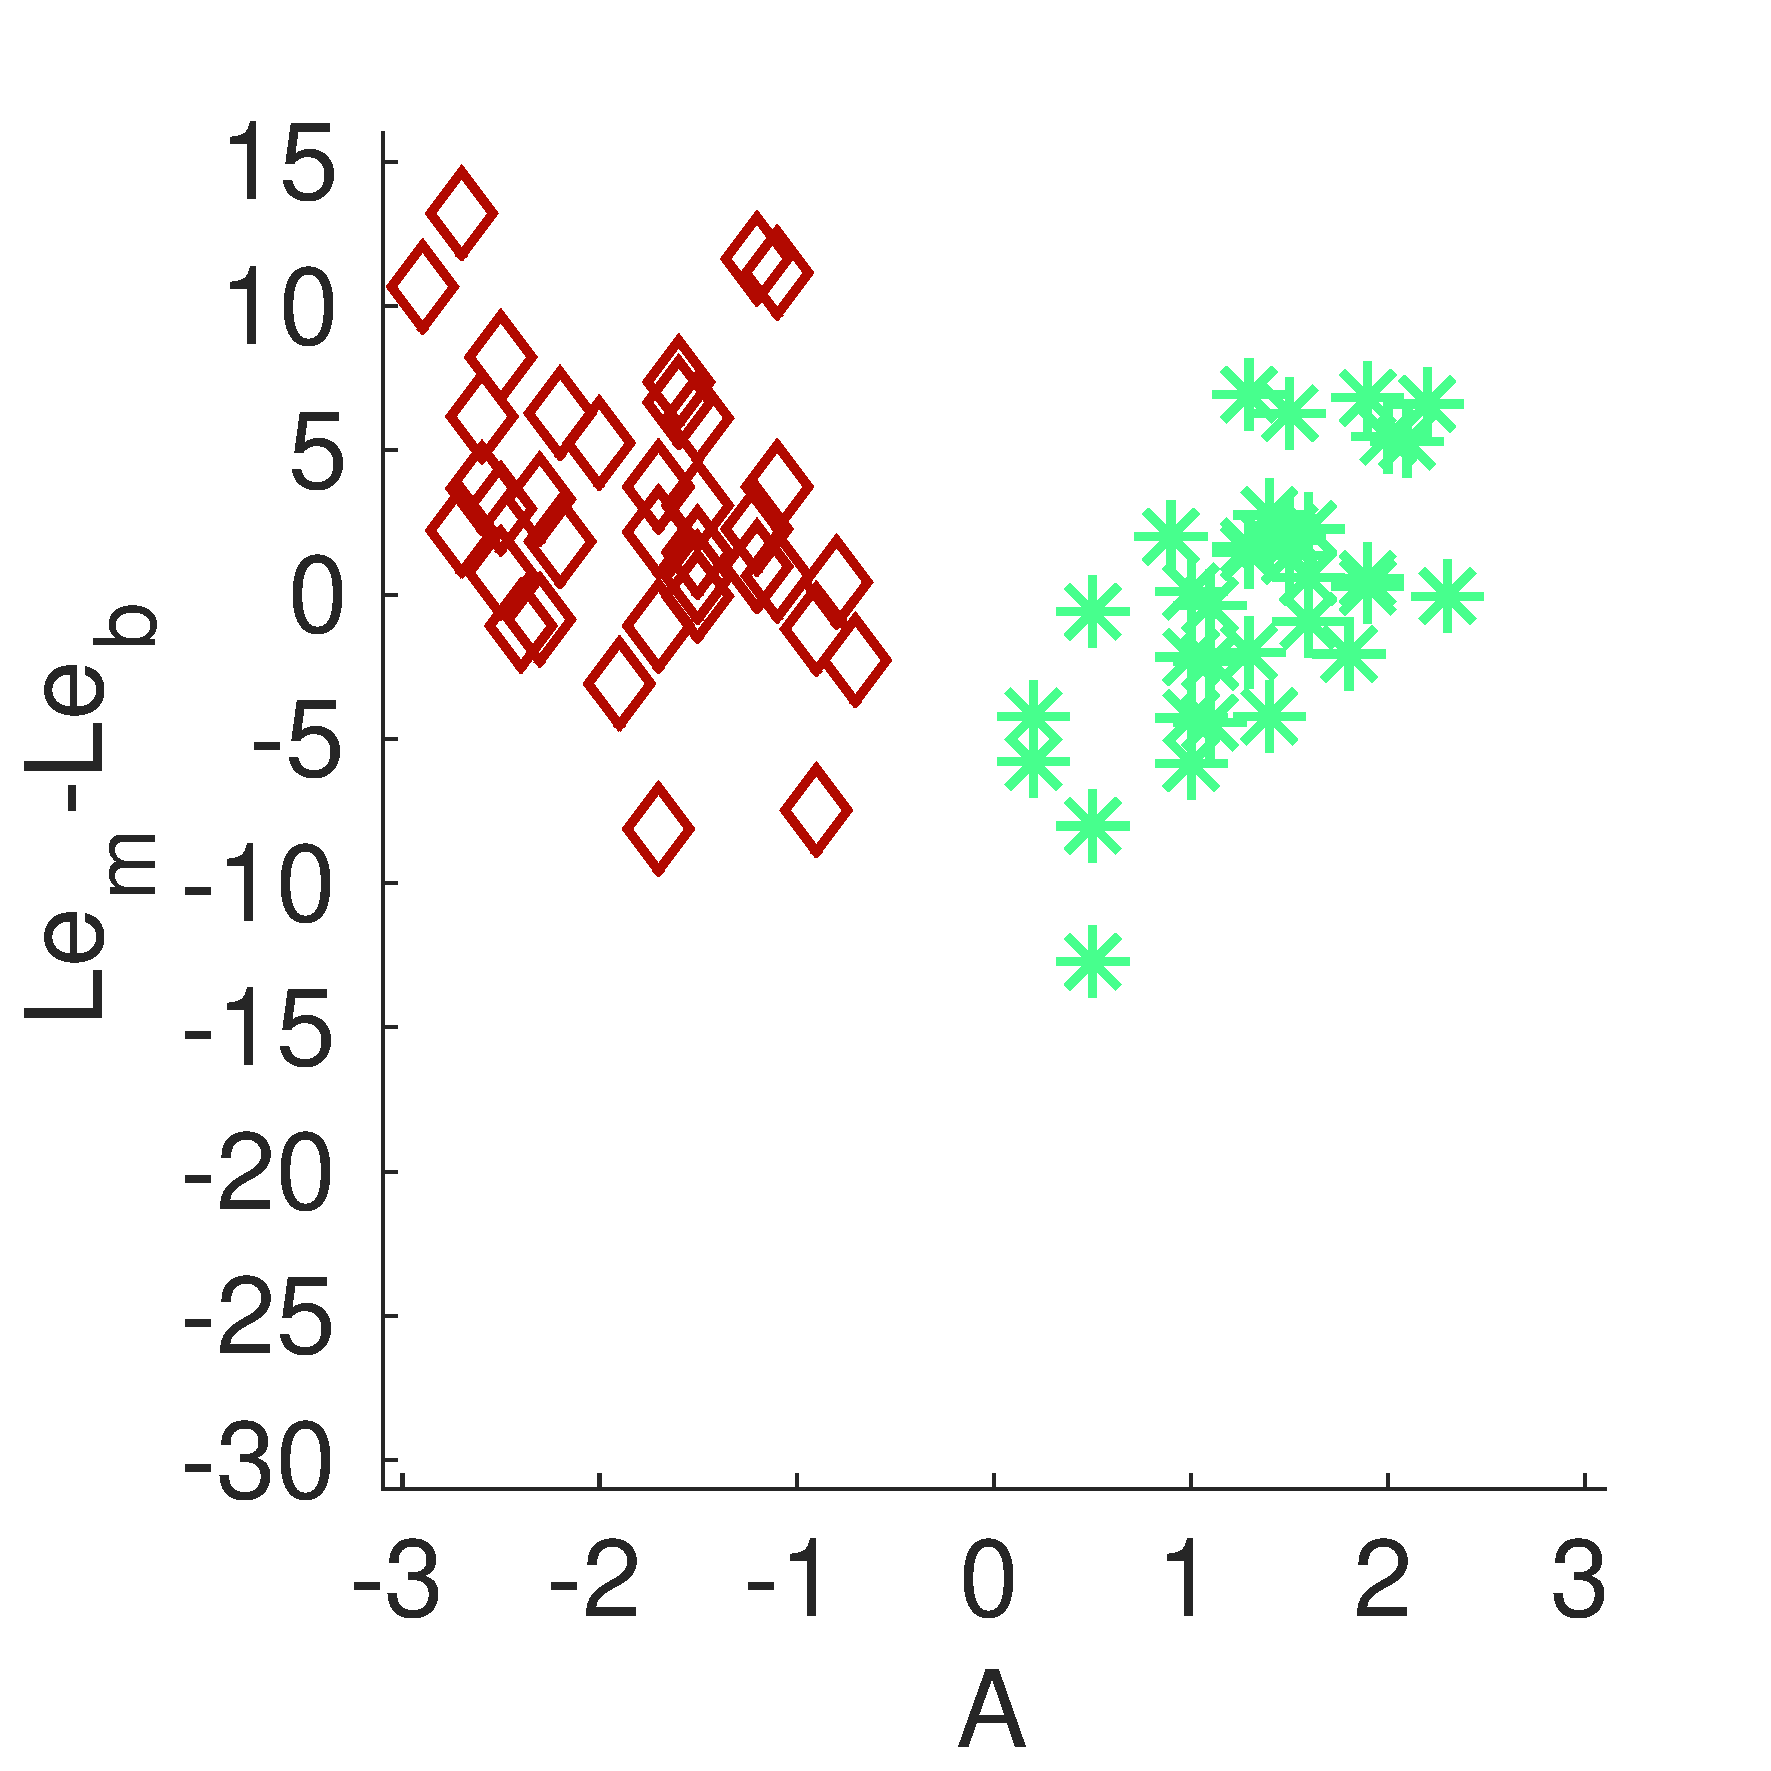
\includegraphics[width=.33\linewidth]{gfxXpUrbanSoundscape/xp_soundlevel_22}\label{fig:soundlevelMarkerDiffe}}
        \subfloat[]
        {\includegraphics[width=.33\linewidth]{gfxXpUrbanSoundscape/xp_soundlevel_24}\label{fig:soundlevelMarkerDifff}}
       \caption[TODO]{TODO}\label{fig:soundlevelMarkerDiff}
\end{figure}

\subsection{Discussions}

\section{Simulation et approche positive}
\label{sec:xp3}

\subsection{Objectif de l'expérience}

\subsection{Planification expérimentale}

\subsection{Données et méthodes d'analyses}

\subsection{Discussions}

\section{Simulation et approche catégorielle}
\label{sec:xp4}

\subsection{Objectif de l'expérience}

\subsection{Planification expérimentale}

\subsection{Données et méthodes d'analyses}

\subsection{Discussions}
%*****************************************
%*****************************************
%*****************************************
%*****************************************
%*****************************************




